\chapter{Efficient Model Differencing of Change-based Models}
\label{ch:model_differencing}

In Chapters \ref{ch:optimised_loading} and \ref{ch:hybrid_model_persistence}, this work proposed two approaches to optimise the loading of change-based model persistence. This chapter presents a method for using change-based persistence in certain circumstances to identify differences between two versions of a model more efficiently than by using state-based persistence. A detailed discussion of the proposed change-based model differencing and its evaluation also is presented in this chapter.

\section{Introduction}
\label{sec:introduction_06}
In modelling and model management, it is common to find that many versions or variants of a model exist. These versions are commonly persisted as snapshots of the model at a given point in time in a state-based format such as XMI. Model differencing activities can be applied to versions of a model to highlight such differences as changes in properties and values, new/deleted elements, etc. However, comparing versions of large file-based
%\footnote{Persisting models in databases involves its own challenges, which have been discussed extensively in the literature. For the rest of this chapter, we are concerned only with file-based models. We return to database-backed model representations in Section \ref{sec:related_work}.}
models in a state-based format can be computationally expensive, since every element of two versions being compared must be loaded into memory to be matched and diffed.

In previous publications from this research \cite{DBLP:conf/models/YohannisKP17,yohannis2018towards,DBLP:conf/models/YohannisRPK18}, change-based model persistence (CBMP) was proposed as an alternative to state-based model persistence of EMF models \cite{steinberg2008emf}. Instead of persisting models as XMI snapshots, models are persisted as a complete history of changes in the proposed approach. We demonstrated the substantial performance benefits of change-based model persistence in terms of saving changes to large models \cite{DBLP:conf/models/YohannisKP17}, and we proposed a method to reduce model loading time compared to naïvely replaying all recorded change events \cite{DBLP:conf/models/YohannisRPK18} to reconstruct the state of a change-based model.
This chapter demonstrates how a change-based representation also enables much more efficient and performant model differencing between versions of the same model. Our experiments, presented in Section \ref{sec:evaluation_6}, demonstrate savings in the order of 90\% for (relatively) small changes made to large models.

This chapter is structured as follows.
Section \ref{sec:runnnig_example_continue} extends the running example from Section \ref{sec:running_example_1} to explaining the differencing approach proposed in this chapter.
Section \ref{sec:state-based_model_differencing} presents the way that state-based model differencing performed in EMF Compare \cite{emfcompare2018developer}.
Section \ref{sec:change_based_approach_for_comparing_models} presents our change-based approach to speed up model differencing and its implementation.
Section \ref{sec:evaluation_6} reports the results of experiments used to evaluate the proposed approach. Section \ref{sec:conclusions_6} concludes this chapter.

\section{Running Example: Part II}
\label{sec:runnnig_example_continue}
In this section, we extend the running example presented in Section \ref{sec:running_example_1}. Using the change-based model persistence presented in Chapter \ref{ch:change_based_model_persistence}, instead of persisting the models in Figure \ref{fig:class_diagram_rpg} only in state-based format, we can also persist the complete history of changes of the models in change-based format.

\vspace{-20pt}
\begin{lstlisting}[style=eol,caption={Change-based representation of the original version in Figure \ref{fig:class_diagram_origin}.},label=lst:cbp_origin]
session "Jane-01"
create character type Class
set character.name from null to "Character"
create attack type Operation
set attack.name from null to "attack"
add attack to character.operations at 0
create gem type Parameter
set gem.name from null to "gem"
add gem to attack.parameters at 0
create target type Parameter
set target.name from null to "target"
add target to attack.parameters at 1
create weapon type Parameter
set weapon.name from null to "weapon"
add weapon to attack.parameters at 2
create troll type Class
set troll.name from null to "Troll"
create giant type class
set giant.name from null to "Giant"
create cast type Operation
set cast.name from null to "smash"
add cast to giant.operations at 0
create knight type Class
set knight.name from null to "Knight"
create smash type Operation
set smash.name from null to "smash"
add smash to knight.operations at 0
create mage type Class
set mage.name from null to "Mage"
\end{lstlisting}

As an example, the complete history of changes made by Jane to construct the original version in Figure \ref{fig:class_diagram_origin} is persisted in a change-based model representation in Listing \ref{lst:cbp_origin}. The change events (Listing \ref{lst:cbp_left}) made by Bob are appended to Jane’s original change events. Thus, the change events that represent Bob’s version (Figure \ref{fig:class_diagram_left}) comprise the original change events and the change events (Listing \ref{lst:cbp_left}) that he made. (Only the appended changes are presented on that list.) The change events that represents Alice’s version (Figure \ref{fig:class_diagram_right}) are presented in Listing \ref{lst:cbp_right}. One clear advantage of change-based model persistence is that, from Listing \ref{lst:cbp_left}, we can immediately know all the changes made by Bob and Alice (starting from line 30), and we can identify all the elements that have been modified since Jane’s version.

\vspace{-20pt}
\begin{lstlisting}[firstnumber=30,style=eol,escapechar=|,caption={The appended events made by Bob to produce Figure \ref{fig:class_diagram_left}.},label=lst:cbp_left]
session "Bob-01"|\label{line:cbp_left_30}|
create leftGen type Generalization|\label{line:cbp_left_31}|
set leftGen.general to character|\label{line:cbp_left_32}|
set troll.generalization to leftGen|\label{line:cbp_left_33}|
set character.name from "Character" to "Hero"|\label{line:cbp_left_34}|
unset troll.generalization from leftGen to null composite l1|\label{line:cbp_left_35}|
set knight.generalization to leftGen composite l1|\label{line:cbp_left_36}|
move target in attack.parameters from 1 to 2|\label{line:cbp_left_37}|
unset cast.name from "cast" to null composite l2|\label{line:cbp_left_38}|
remove cast from giant.operations at 0 composite l2|\label{line:cbp_left_39}|
delete cast composite l2|\label{line:cbp_left_40}|
unset giant.name from "Giant" to null composite l2|\label{line:cbp_left_41}|
delete giant composite l2|\label{line:cbp_left_42}|
set troll.name from "Troll" to "Ogre"|\label{line:cbp_left_43}|
\end{lstlisting}

\vspace{-20pt}
\begin{lstlisting}[firstnumber=30,style=eol,escapechar=|,caption={The appended events made by Alice to produce Figure \ref{fig:class_diagram_right}.},label=lst:cbp_right]
session "Alice-01"|\label{line:cbp_right_30}|
move target in attack.parameters from 1 to 0|\label{line:cbp_right_31}|
remove smash from knight.operations at 0 composite r1|\label{line:cbp_right_32}|
add smash to giant.operations at 0 composite r1|\label{line:cbp_right_33}|
remove cast from giant.operations at 1 composite r2|\label{line:cbp_right_34}|
add cast to mage.operations at 0 composite r2|\label{line:cbp_right_35}|
create rightGen type Generalization|\label{line:cbp_right_36}|
set rightGen.general to character|\label{line:cbp_right_37}|
set troll.generalization to rightGen|\label{line:cbp_right_38}|
set character.name from "Character" to "Hero"|\label{line:cbp_right_39}|
unset troll.generalization from rightGen to null composite r3|\label{line:cbp_right_40}|
set mage.generalization to rightGen composite r3|\label{line:cbp_right_41}|
set troll.name from "Troll" to "Orc"|\label{line:cbp_right_42}|
\end{lstlisting}

Let’s say the complete scenario that produces the models in Figures \ref{fig:class_diagram_origin}, \ref{fig:class_diagram_left}, and \ref{fig:class_diagram_right} as well as Listings \ref{lst:cbp_origin}, \ref{lst:cbp_left}, and \ref{lst:cbp_right} occurred according to the following story.

Jane, as the technical leader, set up the initial model. The events of the initial set-up are recorded in the CBMP in List. \ref{lst:cbp_origin}. She created a class \textsf{Character} that contains an operation \textsf{attack} with three parameters: \textsf{gem}, \textsf{target}, and \textsf{weapon} (lines 2–15). She also created four other classes; \textsf{Troll} (lines 16–17), \textsf{Giant} (lines 18–22), \textsf{Knight} (lines 23–27), and \textsf{Mage} (lines 28–29). Finally, she pushed her work to a change-based version control system. If her work is visualised in state-based format, the model looks like Figure \ref{fig:class_diagram_origin}.

Then Jane assigned work to Bob and Alice. Both of them checked out this project to their own machines. Alice continued the model. She moved parameter \textsf{target} to the first place in operation \textsf{attack}’s parameters, because she thought it was more intuitive for programmers to think about the \textsf{target} before the rest of the parameters (List. \ref{lst:cbp_right}, line 31). She also moved operation \textsf{smash} from class \textsf{Knight} to class \textsf{Giant} and operation \textsf{cast} from class \textsf{Giant} to class \textsf{Mage} as it is more reasonable that they belong to their new classes (lines 32–35). Alice also created a generalisation relationship with ID \textsf{rightGen} from class \textsf{Troll} to class \textsf{Character} (lines 36–39). Bob did the same thing except that his generalisation came with ID \textsf{leftGen} (List. \ref{lst:cbp_left}, lines 31–33).

Later on, Jane informed Alice and Bob that she wanted all good characters to be derived from a general, hero-like class, and the enemy should be Orcs, not Trolls. She also instructed Bob to focus on developing class \textsf{Knight} and Alice on class \textsf{Mage}. As a result, Alice changed the name of class \textsf{Character} from “Character” to “Hero” (the ID of class \textsf{Hero} is still \textsf{character}) (line 39). Again, Bob did the same thing. He also changed the name of class \textsf{Character} from “Character” to “Hero” (line 34). Instead of creating a new generalisation relationship, both of them preferred to move the generalisation relationships that they had created to their assigned classes. Alice moved generalisation \textsf{rightGen} from class \textsf{Troll} to class \textsf{Mage} (lines 40–41), and Bob move generalisation \textsf{leftGen} from class \textsf{Troll} to class \textsf{Knight} (lines 35–36). Bob also moved parameter \textsf{target} in operation \textsf{attack} to the last index, as he thought setting target as the last parameter was intuitive (line 37). Unfortunately, Bob deleted class \text{Giant} accidentally (lines 38–42). The class diagrams of Bob’s and Alice's models are in Figures \ref{fig:class_diagram_left} and \ref{fig:class_diagram_right} respectively. Finally, Alice changed the \textsf{name} of class \textsf{Troll} to “Orc” (line 42) while Bob changed it to “Ogre” (line 43).

In Listings \ref{lst:cbp_right} and \ref{lst:cbp_left}, we also introduce composite events—lines with keyword \textsf{composite}—that represent composite change events.
Composite change events are events that should be treated as one transaction—identified with the same composite ID.
For example, moving an element from one container to another container is a composite event since it consists of two change events:
removing/unsetting the element from its source container and adding/setting it to its target container (lines 40–41 in Listing \ref{lst:cbp_right}).

\section{State-based Model Differencing}
\label{sec:state-based_model_differencing}

Referring to the example in Section \ref{sec:runnnig_example_continue}, Bob decides at some point to compare his model to Alice’s model because he is interested in analysing the differences between their models. Bob uses a model differencing tool to perform state-based model differencing.
In state-based model differencing, comparing models commonly consists of two steps: \emph{matching} and \emph{diffing}.
The matching process establishes similarities between the elements of two models, to determine the elements in the left model that correspond to elements in the right model. Generally, the matching process iterates through all the elements of the models being compared and matches them by their identifiers or through a similarity mechanism \cite{DBLP:conf/sfm/BroschKLSWW12,emfcompare2018developer}. The diffing process then identifies differences between the matched elements \cite{DBLP:conf/sfm/BroschKLSWW12,emfcompare2018developer}.

In our example, the matching process in state-based comparison—as performed by EMF Compare \cite{emfcompare2018developer}—iterates through all the elements of both models and matches them using their identifiers. The matching process yields 10 matches: $m_1$ = (\textsf{character}, \textsf{character}), $m_2$ = (\textsf{attack}, \textsf{attack}), $m_3$ = (\textsf{gem}, \textsf{gem}), $m_4$ = (\textsf{weapon}, \textsf{weapon}), $m_5$ = (\textsf{target}, \textsf{target}), $m_6$ = (\textsf{troll}, \textsf{troll}), $m_7$ = (\textsf{knight}, \textsf{knight}), $m_8$ = (\textsf{smash}, \textsf{smash}), and $m_9$ = (\textsf{mage}, \textsf{mage}), and 3 unmatched elements, $um_1$ = (-, \textsf{giant}), $um_2$ = (-, \textsf{rightGen}), $m_3$ = (-, \textsf{cast}), and $um_4$ = (\textsf{leftGen}, -).

The diffing process then iterates through all the matches and uses an LCS algorithm to identify the differences. During this iteration of the second match $m_2$, the algorithm determines that, to make the left feature \textsf{parameters} equal to the right feature \textsf{parameters}, parameter \textsf{gem} must be moved from index 1 to 0 (diff $ds_1$). It is important to note that the LCS algorithm does not detect the different position of parameter \textsf{weapon}; it only identifies the minimum number of differences which, if all are resolved unidirectionally, can make the two models equal.

In the match $m_6$, the diffing process determines that the classes \textsf{troll} are different in their \textsf{name}. The left \textsf{troll}’s \textsf{name} is “Ogre” while the other \textsf{troll}’s \textsf{name} is “Orc” (diff $ds_2$). In the eighth match $m_8$, the diffing process determines that the containers of operation \textsf{smash} are different. Thus, element \textsf{smash} must be moved from \textsf{knight}’s \textsf{operations} to \textsf{giant}’s \textsf{operations} (diff $ds_3$). For the other matches, the diffing process does not identify any differences.

From the unmatched elements ($um_1$, $um_2$, $um_3$, and $um_4$), the diffing process determines that, to make the left model equal to the right model, class \textsf{giant} must be added to the left model’s resource at index 2 (diff $ds_4$), generalization \textsf{rightGen} must be added to class \textsf{mage}’s \textsf{generalization} (diff $ds_5$), operation \textsf{cast} must be added to class \textsf{mage}’s \textsf{operations} (diff $ds_6$), and generalization \textsf{leftGen} must be removed from class \textsf{knight}’s \textsf{generalization} (diff $ds_7$).

Differences are commonly expressed as a list of changes that must be applied to a target model to make it equal to a reference model. This work treats the left model as a reference model and the right model as the target model. This means that differences are expressed as changes applied to the right model to make it equal to the left model. To express differences, this work uses the following terms: \textsf{LeftContainer}, \textsf{RightContainer}, \textsf{LeftFeature}, \textsf{RightFeature}, \textsf{LeftIndex}, \textsf{RightIndex}, \textsf{LeftValue}, \textsf{RightValue}, and \textsf{Kind}. \textsf{*Container}, \textsf{*Feature}, and \textsf{*Value} are the target element, feature, and value involved in a difference (\textsf{*} symbol can be replaced with \textsf{Left} and \textsf{Right}). \textsf{*Index} is the index of a value in a feature. \textsf{Kind} is the type of difference. It can be one of these types: \textsf{CHANGE}, \textsf{ADD}, \textsf{DELETE}, and \textsf{MOVE}. \textsf{CHANGE} means a pair of single-valued features have different values. \textsf{ADD} indicates that a value does not exist in the right model, thus it requires the addition of the value. \textsf{DELETE} is the opposite of \textsf{ADD}. \textsf{MOVE} indicates that matched elements differ in terms of their containers, containing features, or indexes. A Container is an element that contains a value. A containing feature is a feature owned by a container in which a value is contained. An index is the position of a value in a containing feature.

Based on these definitions, this work can express the result of the diffing process as: $ds_{n}$ = [$LeftContainer_n$, $RightContainer_n$, $LeftFeature_n$, $RightFeature_n$, $LeftIndex_n$, $RightIndex_n$, $LeftValue_n$, $RightValue_n$, $Kind_n$]. Therefore:

$ds_{1}$ = [\textsf{attack}, \textsf{attack}, \textsf{parameters}, \textsf{parameters}, 0, 1, \textsf{gem}, \textsf{gem}, \textsf{MOVE}]\\
$ds_{2}$ = [\textsf{troll}, \textsf{troll}, \textsf{name}, \textsf{name}, 0, 0, “Ogre”, “Orc”, \textsf{CHANGE}]\\
$ds_{3}$ = [\textsf{knight}, \textsf{giant}, \textsf{operations}, \textsf{operations}, 0, 0, \textsf{smash}, \textsf{smash}, \textsf{MOVE}]\\
$ds_{4}$ = [\textsf{resource}, \textsf{resource}, \textsf{null}, \textsf{null}, \textsf{null}, \textsf{null}, \textsf{null}, \textsf{giant}, \textsf{DELETE}]\\
$ds_{5}$ = [\textsf{mage}, \textsf{mage}, \textsf{generalization}, \textsf{generalization}, \textsf{null}, 0, \textsf{null}, \textsf{rightGen}, \textsf{DELETE}] \\
$ds_{6}$ = [\textsf{mage}, \textsf{mage}, \textsf{operations}, \textsf{operations}, \textsf{null}, 0, \textsf{null}, \textsf{cast}, \textsf{DELETE}]\\
$ds_{7}$ = [\textsf{knight}, \textsf{knight}, \textsf{generalization}, \textsf{generalization}, 0, \textsf{null}, \textsf{leftGen}, \textsf{null}, \textsf{ADD}]

We use this information to represent the diffs visually in Figure \ref{fig:xmi_comparison}. We can also transform these diffs into change events that, if the diffs are executed as changes to the right model, they transform it into the left model and generate relevant change events. The change events are presented in Listing \ref{lst:readable_diffs}. Diff $ds_{1}$ produces the change event at line 1 in Listing \ref{lst:readable_diffs}, $ds_{2}$ produces line 2, $ds_{3}$ produces lines 3–4, $ds_{4}$ produces lines 5–7, $ds_{5}$ produces lines 8–10, $ds_{6}$ produces lines 11–13, and $ds_{7}$ produces lines 14–16.

\begin{figure}[ht]
  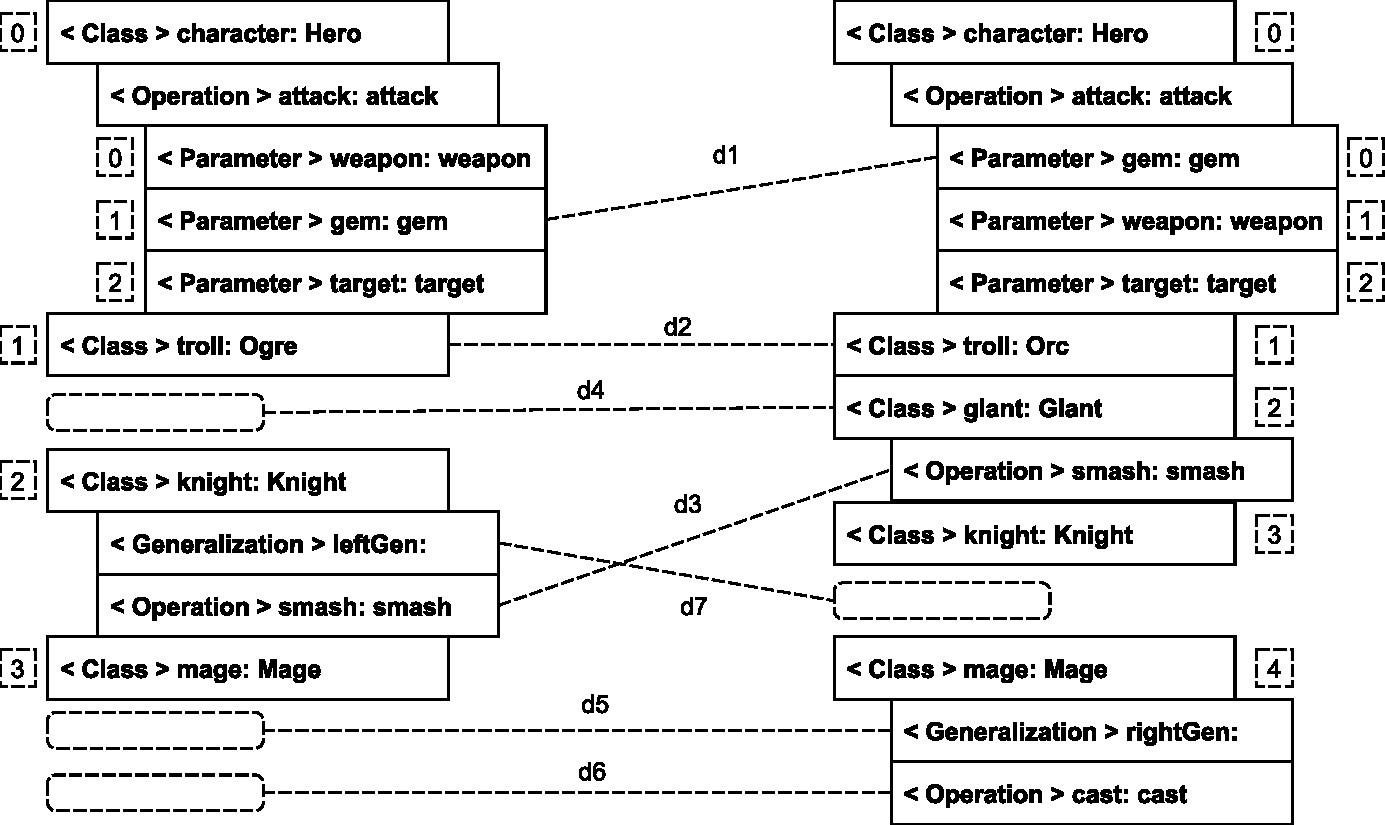
\includegraphics[width=\linewidth]{XmiComparison}
  \caption{A comparison of the left and right models in Listings \ref{lst:xmimodel_left} and \ref{lst:xmimodel_right}.}
  \label{fig:xmi_comparison}
\end{figure}

\vspace{-20pt}
\begin{lstlisting}[firstnumber=1,style=eol,caption={Diffs presented as change events.},label=lst:readable_diffs]
move gem in attack.parameters from 0 to 1
set troll.name from "Orc" to "Ogre"
remove smash from giant.operations at 0 composite c1
add smash to knight.operations at 0 composite c1
unset giant.name from "Giant" to null composite c2
remove giant from resource at 2 composite c2
delete giant composite c2
unset mage.generalization from rightGen to null composite c3
unset rightGen.general from character to null composite c3
delete rightGen composite c3
unset cast.name from "cast" to null composite c4
remove cast from mage.operations composite c4
delete cast composite c4
create leftGen type Generalization composite c5
set knight.generalization from null to leftGen composite c5
set leftGen.general from null to character composite c5
\end{lstlisting}

\section{Change-based Model Differencing}
\label{sec:change_based_approach_for_comparing_models}
Compared to the state-based model conflict detection of EMF Compare, the change-based model conflict detection proposed in this work consists of three phases: event loading, element tree construction, and conflict computation.
Conflict detection is not performed over all the elements of the model, as it is in state-based model differencing. Instead, this approach needs to compare only the last sets of change events of the two models, starting where the lines of the two models are different. A simplified class diagram of this approach \cite{epsilonlabs2019emfcbp} is depicted in Figure \ref{fig:approach_class_diagram}. The three phases are described in detail in the following sections.

\subsection{Event Loading}
\label{sec:event_loading}
In the event loading phase, the implementation loads change events recorded in two change-based model persistence files into memory.
The most important aspect of this phase is the partial loading, as only lines starting where the two files are different are loaded.
Thus, not the whole model needs to be traversed and loaded.
In this case, lines 1–29 in Listing \ref{lst:cbp_origin} are skipped. Only the lines starting with line 30 in Listings \ref{lst:cbp_left} and \ref{lst:cbp_right} are loaded. This yields two partial—left and right—change-event models.

\subsection{Element Tree}
\label{sec:tree_construction}
An element tree is a representation of the changes of model elements in the source and reference models. It contains detailed information about elements and their properties. It contains information similar to that captured in change lists in state-based model persistence, but it also provides more information about the changes. For example, the element tree can keep track of a feature’s old value and an element/value’s indexes inside multi-valued properties. The element tree contains only the partial states of affected elements of the original, left, and right models as depicted in Figures \ref{fig:left_element_tree_diagram} and \ref{fig:right_element_tree_diagram}.

To better understand the construction of an element tree from change events, we use the following running example using both change events in Listings \ref{lst:cbp_left} and \ref{lst:cbp_right}. We start from the left change events.

\subsubsection{Left Side}\label{sec:left_side}
In the first change event in Listing \ref{lst:cbp_left} at line \ref{line:cbp_left_30}, the change event is a \textsf{session} event. It indicates that all the following change events until the final line or next \textsf{session} event are persisted in one batch when they are saved. At line \ref{line:cbp_left_31}, we can see that Bob created a \textsf{Generalization} with ID \textsf{leftGen}. Thus, in \textsf{elementTree}, an element with ID \textsf{leftGen} also is created. To indicate that an element is newly created in the session, we put a ‘+’ sign at the left lower box of element \textsf{leftGen} in Figure \ref{fig:left_element_tree_diagram}.

\begin{landscape}
  \begin{figure}
    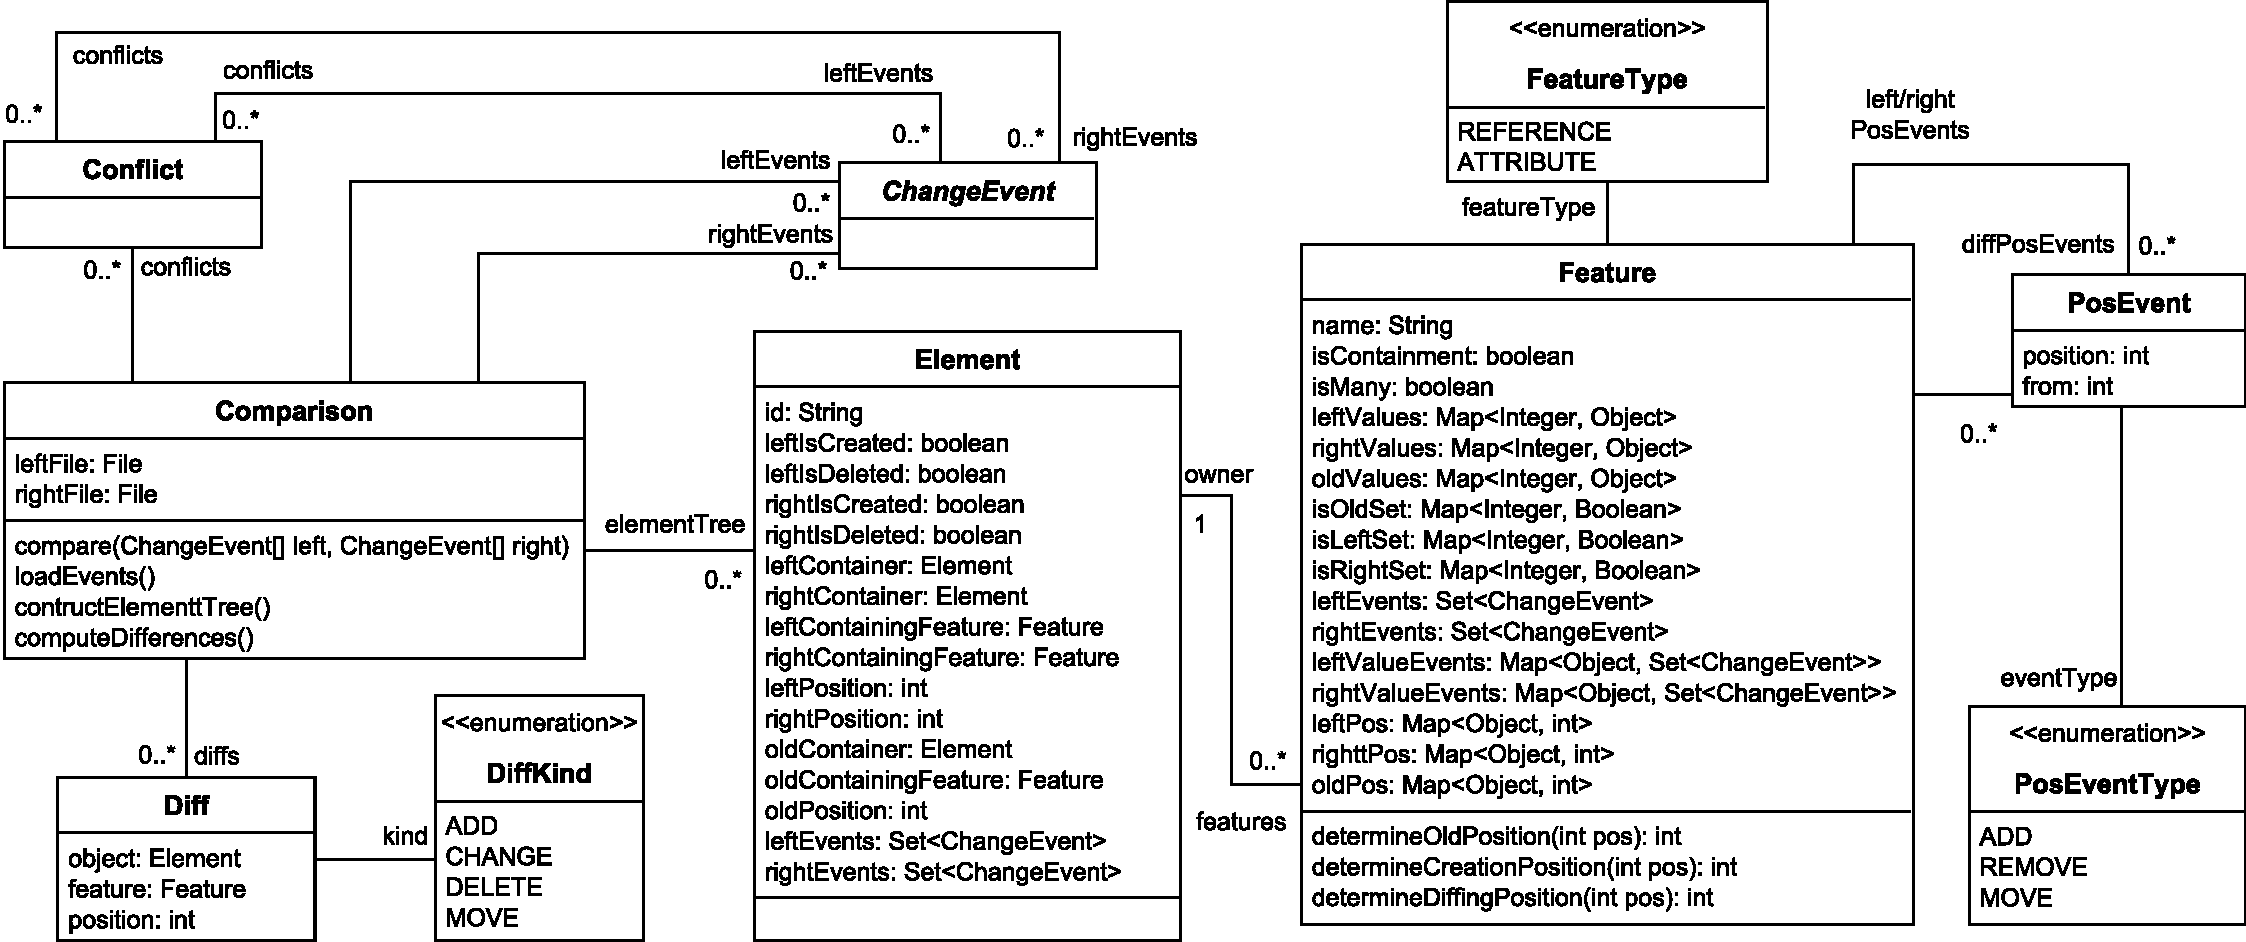
\includegraphics[width=\linewidth]{TreeClassDiagram}
    \caption{A class diagram showing the core components of the change-based approach to speed up model differencing and conflict detection.}
    \label{fig:approach_class_diagram}
  \end{figure}
\end{landscape}

\begin{figure}[ht]
  \centering
  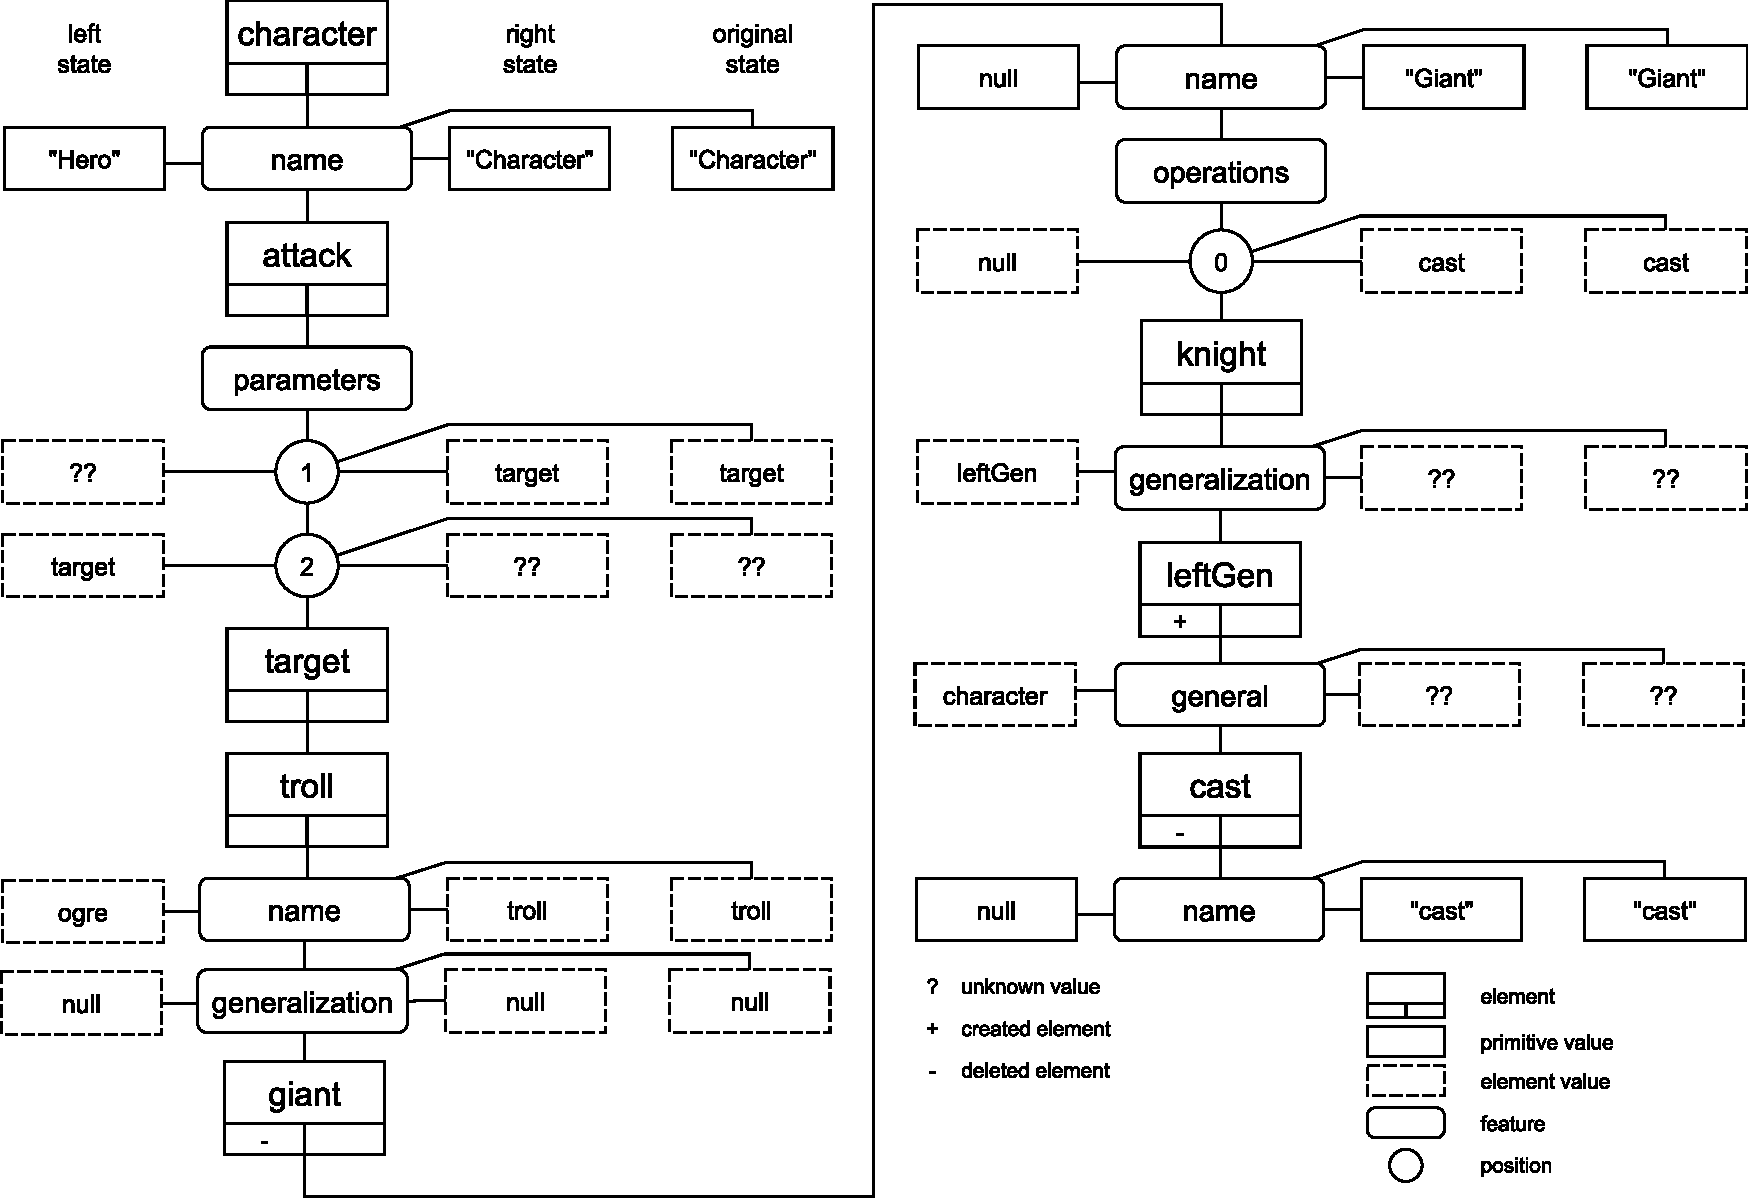
\includegraphics[width=\linewidth]{element_tree_game_left}
  \caption{An element tree constructed from information in CBPs in Listing \ref{lst:cbp_left} (left change events only).}
  \label{fig:left_element_tree_diagram}
\end{figure}

At line \ref{line:cbp_left_32}, the feature \textsf{general} of \textsf{leftGen} is set to \textsf{character}. From the change event, we can recognise that \textsf{character} existed in the previous version since it has not been created in the current editing session. Thus, we create an element with ID \textsf{character} and the feature \textsf{general} of \textsf{leftGen} and put them in \textsf{elementTree}. We then set the value of \textsf{general} to \textsf{character} on the left side. We follow the same routine with \textsf{troll} and \textsf{generalization} at line \ref{line:cbp_left_33}, adding element \textsf{troll} and feature \textsf{generalization} to \textsf{elementTree} and setting the value of feature \textsf{generalization} to \textsf{leftGen} on the left side of the \textsf{elementTree}.

The change event at line \ref{line:cbp_left_34} changes \textsf{character}’s \textsf{name} from “Character” to “Hero”. From the change event, we can see that \textsf{character} existed before. Thus, we create element \textsf{character} and feature \textsf{name} into \textsf{elementTree}. We also set the value of \textsf{name} to “Hero” on the left side. Since this set change event is the first event for \textsf{character}’s \textsf{name}, we can infer that the original value of \textsf{name} is “Character”. Thus, we set \textsf{name}’s value to “Character” on the original side. The value of \textsf{name} on the right side also is set to “Character”, but it will be modified later when we process the right change events (Alice’s change events) if there is any change event that affects it. The same routine is applied when we process the change event at line \ref{line:cbp_left_43} later.

Lines \ref{line:cbp_left_35} and \ref{line:cbp_left_36} are the change events of composite move event \textsf{l1}. Element \textsf{leftGen} is removed (unset) from \textsf{troll}’s \textsf{generalization} and is assigned (set) to \textsf{knight}’s \textsf{generalization}. From these change events, we can see that element \textsf{knight} also existed in the original version. Thus, we add it into \textsf{elementTree} together with its \textsf{generalization} feature. Element \textsf{troll} and its \textsf{generalization} feature are not added into \textsf{elementTree} any more since they were added when processing line \ref{line:cbp_left_33}. In \textsf{elementTree}, we set \textsf{troll}’s \textsf{generalization} to null since element \textsf{leftGen} is moved to \textsf{knight}’s \textsf{generalization}.

At line \ref{line:cbp_left_37}, \textsf{target} is moved from index 1 to 2 in \textsf{attack}’s \textsf{parameters}. From the change event, we can see that element \textsf{target} has been contained in \textsf{attack}’s \textsf{parameters} at index 1 since the original version. Thus, we put element \textsf{target} and element \textsf{attack} and its \textsf{parameters} feature into \textsf{elementTree}. We also create a map on the left side with a key ‘2’ and a value that points to element \textsf{target} for feature \textsf{parameters}, indicating \textsf{target} is at index 2 in the left version. Since it is the first change event that moves \textsf{target}, we can decide that \textsf{target} is at index 1 in the original version. Thus, we create another map on the original side a map on the left side with a key ‘1’ and a value that also points to \textsf{target}. We also perform this routine to the right side of feature \textsf{parameters}, creating a map with a key ‘1’ and a value that also points to \textsf{target}. It will be modified later when we process the right change events (Alice’s change events) if there is any change event that affects the index of \textsf{target}.

Lines \ref{line:cbp_left_38} to \ref{line:cbp_left_42} are the change events of composite delete event \textsf{l2}; a deletion of element \textsf{giant}.
A deletion of an element unsets all the features of that element and its sub-elements, removes the sub-elements from their containers, and deletes the element and sub-elements from the model.
As can be seen, the value of \textsf{cast}’s \textsf{name} is unset from “cast” to null at line \ref{line:cbp_left_38}. From the change event, we know that cast has existed since the original version. Thus, we add element \textsf{cast} and its feature \textsf{name} to \textsf{elementTree} and set its value null on the left side and “cast” on the origin and right sides.

At line \ref{line:cbp_left_39}, \textsf{cast} is removed from \textsf{giant}’s \textsf{operations} at index 0. From it, we can see that \textsf{giant} and its feature \textsf{operations} exist, and \textsf{cast} is contained in \textsf{giant}’s \textsf{operations} at index 0 in the original version. Thus, we create element \textsf{giant} and its feature \textsf{operations} in \textsf{elementTree}. Three maps also are created in \textsf{operations} for the three sides. Each map contains a key ‘0’, indicating index, and a value that points to element \textsf{cast}—except on the left side the value is null since \textsf{cast} is removed from \textsf{giant}’s \textsf{operations}. The deletion of \textsf{cast} at line \ref{line:cbp_left_40} marks \textsf{cast} in \textsf{elementTree} with a ‘-’ sign on the left side to indicate that the element is deleted from the model in the left version.

Change event at line \ref{line:cbp_left_41} is similar to change event at line \ref{line:cbp_left_38}, except that it is applied to \textsf{giant}’s \textsf{name}. Since \textsf{giant} has existed in \textsf{elementTree}, only the feature \textsf{name} is added. Its value is set to null on the left side and “Giant” on the origin and right sides. The deletion of \textsf{giant} at line \ref{line:cbp_left_42} marks \textsf{giant} in \textsf{elementTree} with a ‘-’ sign to indicate that the element is deleted from the model in the left version.

Figure \ref{fig:left_element_tree_diagram} illustrates the state of the \textsf{elementTree} after all left change events have been processed. As can be seen, the \textsf{elementTree} exhibits the partial states of the original, left, and right models at once.

\subsubsection{Right Side}\label{sec:right_side}
In Listing \ref{lst:cbp_right}, similar to processing the left change events, the processing of the right change events (Alice’s version) starts with processing the session event at line \ref{line:cbp_right_30}. At line \ref{line:cbp_right_31}, \textsf{target} is moved from index 1 to 0 in \textsf{attack}’s \textsf{parameters}. Since the index of \textsf{target} is already determined when processing the change event, we determine the index of \textsf{target} only on the right side. We unset the value of key ‘1’ on the right side to null and create a new key ‘0’ that maps its value to \textsf{target}.

\begin{figure}[ht]
  \centering
  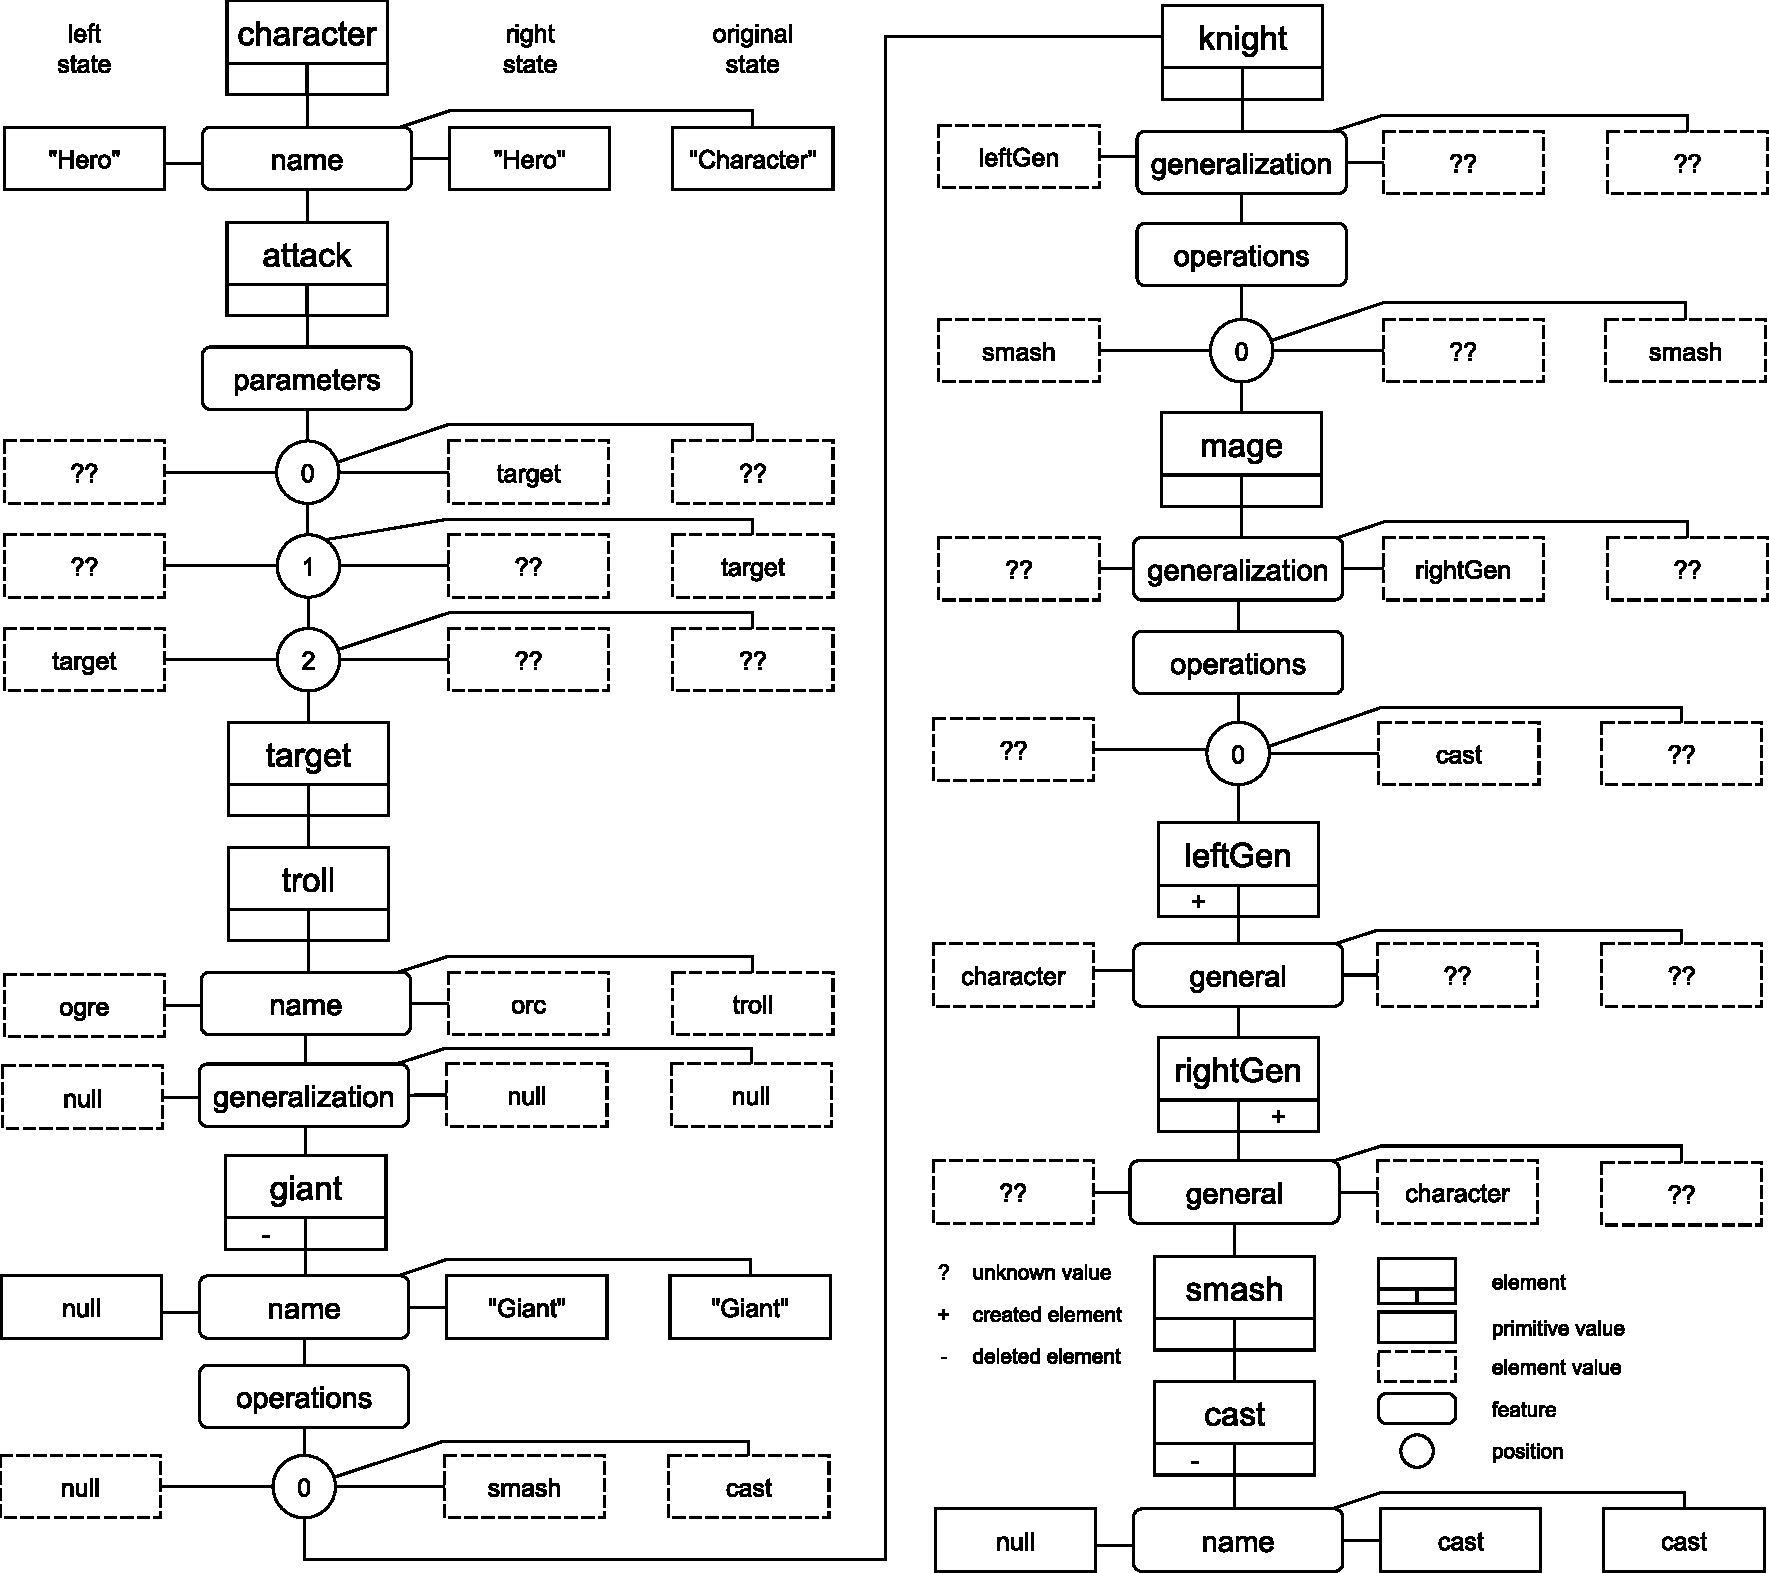
\includegraphics[width=\linewidth]{element_tree_game_right}
  \caption{An element tree constructed from information in CBPs in Listings \ref{lst:cbp_left} and \ref{lst:cbp_right} (all left and right change events).}
  \label{fig:right_element_tree_diagram}
\end{figure}

Composite move event \textsf{r1} at lines \ref{line:cbp_right_32} and \ref{line:cbp_right_33} moves \textsf{smash} from \textsf{knight}’s \textsf{operations} to \textsf{giant}’s \textsf{operations}. From this move event, we can see that \textsf{smash} is no longer in \textsf{knight}’s \textsf{operations}; it is contained in \textsf{giant}’s \textsf{operations} on the right side. Element \textsf{smash} has never existed in \textsf{elementTree}. So, we create and add \textsf{smash} to \textsf{knight}’s \textsf{operations} at index 0 on the origin side and to \textsf{giant}’s \textsf{operations} at index 0 on the right side. Since \textsf{smash} is not modified on the left side and no other change events applied to \textsf{knight}’s \textsf{operations}, we can determine that \textsf{smash} is at index 0 in \textsf{giant}’s \textsf{operations} on the left side.

Lines \ref{line:cbp_right_34} to \ref{line:cbp_right_35} are change events that constitute composite move event \textsf{r2}. This event moves \textsf{cast} from \textsf{giant}’s \textsf{operations} to \textsf{mage}’s \textsf{operations}. From this move event, we can see that \textsf{cast} is no longer in \textsf{giant}’s \textsf{operations} but now exists in \textsf{mage}’s \textsf{operations} on the right side. Element \textsf{mage} and its feature \textsf{operations} have never existed in \textsf{elementTree}. So, we create and add them to \textsf{elementTree} and add \textsf{cast} to \textsf{mage}’s \textsf{operations} on the right side.

At line \ref{line:cbp_right_36}, we can see that Alice created a \textsf{Generalization} with ID \textsf{rightGen}. Thus, in \textsf{elementTree}, an element with ID \textsf{rightGen} is created. Since it has just been created in the active session, the element is marked with a ‘+’ sign in \textsf{elementTree} on the right side. At line \ref{line:cbp_right_37}, we can also see that feature \textsf{general} should be added to \textsf{rightGen} in \textsf{elementTree} and the value is set to \textsf{character} on the right side. We also set \textsf{mage}’s \textsf{operations} to \textsf{rightGen} on the right side of \textsf{elementTree} according to the change event at line \ref{line:cbp_right_38}.

Change event at line \ref{line:cbp_right_39} changes \textsf{character}’s \textsf{name} from “Character” to “Hero”. Since \textsf{character} and its feature \textsf{name} already exist in \textsf{elementTree}, we set \textsf{name}’s value to “Hero” only on the right side. The original value was already assigned when processing left change events. We apply the same routine when processing the change event at line \ref{line:cbp_right_42} later.



Composite move event \textsf{r3} at lines \ref{line:cbp_right_40} and \ref{line:cbp_right_41} moves \textsf{rightGen} from \textsf{troll}’s \textsf{generalization} to \textsf{mage}’s \textsf{generalization}. From this move event, on the right side, we can see that \textsf{rightGen} is no longer in \textsf{troll}’s \textsf{generalization} but exists in \textsf{mage}’s \textsf{generalization}. Since it is the first time \textsf{mage}’s \textsf{generalization} is modified, we create and add the feature to \textsf{mage} in \textsf{elementTree}. On the right side of \textsf{elementTree}, we unset \textsf{troll}’s \textsf{generalization} to null and assign \textsf{rightGen} to \textsf{mage}’s \textsf{generalization}.

Figure \ref{fig:right_element_tree_diagram} exhibits the state of the \textsf{elementTree} after both sides’ change events have been processed.

\subsubsection{Construction Procedure}\label{sec:construction_procedure}

The construction of \textsf{elementTree} follows the steps shown in Figure \ref{fig:tree_construction}. First, the partial state $S_{L}$ of the left model in the \textsf{elementTree} is constructed based on the information retrieved from the left change events (step 1). We denote this information as $I_{LL}$. We can also construct the partial state $S_{O}$ of the original model using the information about the original state contained in the left change events $I_{OL}$ (step 2). The information $I_{OL}$ allows us to construct the initial partial state $S_{R}$ of the right model (step 3). Similarly, using the information from the right change events $I_{RR}$, we update the partial right state $S_{R}$, which was initialised before using the information $I_{OL}$ (step 4), implying that $I_{OL} \cup I_{RR} \rightarrow S_{R}$. Also, information about the original model from the right change events $I_{OR}$ is used to update the original state (step 5). Thus, we have constructed a partial state of the original model using information from both left and right sides, $I_{OL} \cup I_{OR} \rightarrow S_{O}$. Finally, we also use the information $I_{OR}$ to update the partial state of the left model (step 6), implying that $I_{LL} \cup I_{OR} \rightarrow S_{L}$.

\begin{figure}[ht]
  \centering
  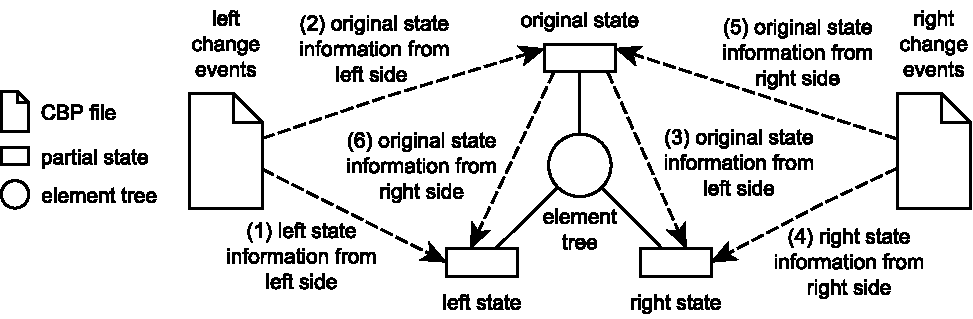
\includegraphics[width=\linewidth]{TreeConstruction}
  \caption{Steps in Element Tree construction.}
  \label{fig:tree_construction}
\end{figure}

Algorithm \ref{alg:element_tree} describes the steps presented in Figure \ref{fig:tree_construction} in a generic fashion. It iterates through all of a model’s change events and uses the information contained in them to construct the relevant partial state. The choice to begin with left or right change events depends on the \textsf{Side} enumeration value—\textsf{left} or \textsf{right}—passed through the parameter \textsf{side} (the second input parameter). In our implementation, we process the left side first by default. The algorithm also receives an input of the change events \textsf{events} that are to be iterated and the element tree \textsf{elementTree} that has been instantiated. Then it returns the \textsf{elementTree} as output after updating it.

For each \textsf{event} in the \textsf{events}, we collect information needed to build up \textsf{elementTree} (lines 3–9), such as \textsf{targetElement}, \textsf{feature}, \textsf{value}, \textsf{previousValue}, \textsf{index}, and \textsf{previousIndex}. The \textsf{targetElement} is the element modified by a change event (e.g., \textsf{character} and \textsf{giant} in Listing \ref{lst:cbp_left}). This \textsf{targetElement}—an instance of class Element in Figure \ref{fig:approach_class_diagram}—is retrieved from the \textsf{elementTree} if it already exists. Otherwise, a new element is created and added to the \textsf{elementTree} (line 3). In this step we also set the flags \textsf{*IsCreated} and \textsf{*IsDeleted} of the element in Figure \ref{fig:approach_class_diagram}. For example, if the type of the event is \textsf{create} then \textsf{*IsCreated} is set to \textsf{true}. The \textsf{feature}—an instance of class Feature in Figure \ref{fig:approach_class_diagram}—represents the target element’s feature (e.g., \textsf{name} and \textsf{operations} in Listing \ref{lst:cbp_right}) modified by a change event. It is retrieved from the \textsf{targetElement}’s feature list, and a new one is created and added to the \textsf{targetElement}’s feature list if the feature does exist (line 5).

\IncMargin{1.5em}
\begin{algorithm}[H]
  \begin{footnotesize}
    \SetKwInOut{Input}{input}
    \SetKwInOut{Output}{output}
    \Input{a list of ChangeEvent $events$}
    \Input{an enumeration of Side $side$}
    \Input{an instance of ElementTree $elementTree$}
    \Output{an instance of ElementTree $elementTree$}
    \SetKwBlock{Beginn}{beginn}{ende}
    \Begin{
      \ForEach{$event$ in $events$}{
        $targetElement$ $\leftarrow$ getOrCreateNewTargetElement($event$, $elementTree$)\;
        $feature$ $\leftarrow$ getOrCreateNewFeature($event$, $targetElement$)\;
        $value$ $\leftarrow$ getValue($event$)\;
        $previousValue$ $\leftarrow$ getPreviousValue($event$)\;
        $index$ $\leftarrow$ getIndex($event$)\;
        $previousIndex$ $\leftarrow$ getPreviousIndex($event$)\;
        $featureEventList$ $\leftarrow$ getFeatureEventList($feature$, $side$)\;
        
        \BlankLine
        \tcp{put all values to their proper indexes}
        updateTree($targetElement$, $feature$, $value$, $index$, $side$)\;
        $oldIndexes$ $\leftarrow$ calculateOldIndex($featureEventList$, $previousIndex$, $side$)\;
        \If{\Not isCreated($value$, $side$) \AndA \Not isOldValueSet($feature$, $previousValue$, $previousIndex$, $side$)} {
          setOldValue($feature$, $previousValue$, $oldIndex$, $side$)\;
          $oppositeFeatureEventList$ $\leftarrow$ getOppositeFeatureEventList($feature$, $side$)\;
          $oppositeIndex$ $\leftarrow$ calculateOppositeIndex($oppositeFeatureEventList$, $oldIndex$, $side$)\;
          \If{\Not isDeleted($value$, $side$) \AndA \Not isOppositeSideValueSet($feature$, $value$, $oppositeIndex$, $side$)} {
            setOppositeSideValue($feature$, $value$, $oppositeIndex$, $side$)\;
          }
        }
        
        addEventToFeatureEventList($event$, $featureEventList$)\;
        
      }
      \Return{$elementTree$}\;
    }
  \end{footnotesize}
  \caption{Algorithm to construct an element tree from events.}
  \label{alg:element_tree}
\end{algorithm}
\DecMargin{1.5em}

The \textsf{value} is the value assigned to the feature in a change event (line 5, Algorithm \ref{alg:element_tree}). The \textsf{value} can be a type of \textsf{Element} (e.g., element \textsf{leftGen} line \ref{line:cbp_left_36} in Listing \ref{lst:cbp_left}) or primitive (e.g., the string “Hero” at line \ref{line:cbp_left_34} in Listing \ref{lst:cbp_left}). The \textsf{previousValue} represents the previous value of the modified feature (line 6, Algorithm \ref{alg:element_tree}). The \textsf{previousValue} is not defined if no previous value has been assigned. For \textsf{value} and \textsf{previousValue} with type \textsf{Element}, the elements they represent are retrieved from the \textsf{elementTree}, and if they do not exist, new instances are created. If the type is primitive, the value is treated as it is. Not every change event has a \textsf{value}, particularly events with type \textsf{create}
or \textsf{delete}, which modify only a target element not an element feature.

The \textsf{index} is the index assigned by a change event to a value in a feature, while \textsf{previousIndex} is the previous index of the value (lines 7–8, Algorithm \ref{alg:element_tree}). In one change event, we can get both \textsf{index} and \textsf{previousIndex} or only one of them, depending on the type of the change event. For example, we can determine that the \textsf{index} of \textsf{cast} is 0 (line \ref{line:cbp_right_35} in Listing \ref{lst:cbp_right}) because the change event type is \textsf{add}. In a \textsf{remove} change event, we can get only the \textsf{previousIndex} of \textsf{cast}, which is 1 (line \ref{line:cbp_right_35} in Listing \ref{lst:cbp_right}), because the element does not exist anymore in the left model. We can obtain both of them only in a \textsf{move} change event as an element is moved from a previous index to a new one (line \ref{line:cbp_right_31} in Listing \ref{lst:cbp_right}). For a single-valued feature, the \textsf{index} and \textsf{previousIndex} are always 0, because the feature can contain only a single value.

At line 9, we retrieve the \textsf{featureEventList} from the \textsf{feature} to be added later with the current \textsf{event} (line 19). The \textsf{featureEventList} is a list—a history—of change events that have been processed that are specific to the \textsf{feature} on the selected \textsf{side}. Using the obtained \textsf{targetElement}, \textsf{feature}, \textsf{value}, and \textsf{index}, the process then updates the state of the \textsf{elementTree} on the selected \textsf{side} (line 10). After that, it calculates the original index of a value, using the \textsf{featureEventList} and \textsf{previousIndex} (line 11). If the value at \textsf{oldIndex} in the \textsf{feature} has not been set, then the algorithm sets the \textsf{feature} with the \textsf{previousValue} at the \textsf{oldIndex} in the partial state of the original model (lines 12–13). At lines 14–18, the algorithm does the same thing to the opposite side—if the current \textsf{side} is \textsf{left} then it is \textsf{right}.

\subsection{Diff Computation}
\label{sec:diff_computation}
Using the \textsf{elementTree} presented in Figure \ref{fig:right_element_tree_diagram}, we can determine the difference between the left and right models without having to compare all their elements and features. After the \textsf{elementTree} has been constructed, we iterate through elements and features of the \textsf{elementTree} and use the flags, containers, containing features, and indexes on both sides of each element and value to identify differences between the left and right models. We follow the steps in Algorithm \ref{alg:diff_calculation}. The algorithm visits each element and every index of each feature (lines 3–5). At every index, it retrieves the \textsf{leftValue} and \textsf{rightValue} (lines 5–7), passing these, together with the \textsf{element}, \textsf{feature}, and \textsf{index} to a function \textsf{identifyDiffUsingRules} (line 8). The function uses a set of pre-defined rules to identify the differences \textsf{diffs} based on the states of flags of an element, flags and attributes of the element’s feature, values of the feature, and indexes of the values. The obtained \textsf{diffs} are then added to the overall list of differences \textsf{diffList} which is output (line 8–9, 13).

\IncMargin{1.5em}
\begin{algorithm}[H]
  \begin{footnotesize}
    \SetKwInOut{Input}{input}
    \SetKwInOut{Output}{output}
    \Input{an instance of ElementTree $elementTree$}
    \Begin{
      $diffList$ $\leftarrow$ DiffList()\;
      \ForEach{$element$ \In $elementTree$}{
        \ForEach{$feature$ \In getFeatures($element$)}{
          \ForEach{$index$ \In getIndexes($feature$)}{
            $leftValue$ $\leftarrow$ getLeftValue($feature$, $index$)\;
            $rightValue$ $\leftarrow$ getRightValue($feature$, $index$)\;
            \BlankLine
            \tcp{rules starts from here}
            $diffs$ $\leftarrow$ identifyDiffUsingRules($element$, $feature$, $leftValue$, $rightValue$, $index$)\;
            addToDiffList($diffs$,$diffList$)\;
          }
        }
      }
      \Return{$diffList$}\;
    }
  \end{footnotesize}
  \caption{Algorithm to determine differences.}
  \label{alg:diff_calculation}
\end{algorithm}
\DecMargin{1.5em}

We illustrate the principles and the use of rules by discussing the rules used to identify differences in the running example. These can be found in Algorithm \ref{alg:diff_rules}. The algorithm is the breakdown of the function \textsf{identifyDiffUsingRules} in Algorithm \ref{alg:diff_calculation}. As previously stated, it is important to remember that we use the left model as a reference, which means the differences are presented as changes that transform the right model to become equal to the left model.

\IncMargin{1.5em}
\begin{algorithm}[]
  \begin{footnotesize}
    \SetKwInOut{Input}{input}
    \SetKwInOut{Output}{output}
    \Input{an Element $element$, a Feature $feature$, a variable $leftValue$, a variable $rightValue$, an Integer $index$}
    \Output{a List of Diff $diffs$}
    $diffs$ $\leftarrow$ createDiffList()\;
    \tcp{...}
    \tcp{Rule 1: a rule to determine a change of a single-valued attribute}
    \If{getType($feature$) \Is Attribute \AndA isSingleValued($feature$) \AndA leftValue <> rightValue \AndA \Not leftIsCreated($element$) \AndA \Not leftIsDeleted($element$) \AndA \Not rightIsCreated($element$) \AndA \Not rightIsDeleted($element$)}{
      $diff$ $\leftarrow$ createNewDiff($element$, $element$, $feature$, $feature$, $index$, $index$, $leftValue$, $rightValue$, DifferenceType.CHANGE)\;
      addDiffToDiffList($diff$, $diffs$)\;
    }
    \tcp{Rule 2: A rule to determine movement of an element for right value (the left value has its own rule)}
    \If{getType($feature$) \Is Containment \AndA \Not isNull($rightValue$) \AndA \Not leftIsCreated($rightValue$) \AndA \Not leftIsDeleted($rightValue$) \AndA \Not rightIsCreated($rightValue$) \AndA \Not rightIsDeleted($rightValue$) \AndA (getLeftContainer($rightValue$) <> getRightContainer($rightValue$) \Or getLeftFeature($rightValue$) <> getRightFeature($rightValue$) \Or getLeftIndex($rightValue$) <> getRightIndex($rightValue$))}{
      $diff$ $\leftarrow$ createNewDiff(getLeftContainer($rightValue$), getRightContainer($rightValue$), getLeftFeature($rightValue$), getRightFeature($rightValue$), getLeftIndex($rightValue$), getRightIndex($rightValue$), $rightValue$, $rightValue$, DifferenceType.MOVE)\;
      addDiffToDiffList($diff$, $diffs$)\;
    }
    \tcp{Rule 3: The first of two rules to determine the deletion of an element}
    \If{getType($feature$) \Is Containment \AndA \Not leftIsCreated($rightValue$) \AndA leftIsDeleted($rightValue$) \AndA \Not rightIsCreated($rightValue$) \AndA \Not rightIsDeleted($rightValue$) }{
      createNewDiff(getLeftContainer($rightValue$), getRightContainer($rightValue$), getLeftFeature($rightValue$), getRightFeature($rightValue$), null, getRightIndex($rightValue$), null, $rightValue$, DifferenceType.DELETE)\;
      addDiffToDiffList($diff$, $diffs$)\;
    }
    \tcp{...}
    \tcp{continue to part 2}
  \end{footnotesize}
  \caption{Some rules to determine differences (part 1).}
  \label{alg:diff_rules}
\end{algorithm}
\DecMargin{1.5em}

The first rule (Rule 1) in Algorithm \ref{alg:diff_rules} is to identify changes in single-valued attributes. A feature must be of type \textsf{attribute}, both side values must be different, and the element should have not been created or deleted in both models. The second rule (Rule 2) identifies whether an element is in a different location in the two models. The element must not have been deleted, and it must exist from the previous version—the original model. Also, the containers, containing features, or indexes of the element must be different on the two sides. The third rule (Rule 3) identifies the deletion of an element. If an element in the left model is not created but exists in the model, it means that the element has existed since the previous version—the original model. This also means that the element also exists in the right model, unless it has been deleted. Thus, to make the right model equal to the left model, the element must be deleted in the right model as well.

\IncMargin{1.5em}
\begin{algorithm}[H]
  \begin{footnotesize}
    \tcp{continuation of part 1}
    \tcp{...}
    \tcp{Rule 4: The second of two rules to determine deletion of an element}
    \If{getType($feature$) \Is Containment \AndA \Not leftIsCreated($rightValue$) \AndA \Not leftIsDeleted($rightValue$) \AndA rightIsCreated($rightValue$) \AndA rightIsDeleted($rightValue$) }{
      createNewDiff(getLeftContainer($rightValue$), getRightContainer($rightValue$), getLeftFeature($rightValue$), getRightFeature($rightValue$), null, getRightIndex(rightValue), null, $rightValue$, DifferenceType.DELETE)\;
      addDiffToDiffList($diff$, $diffs$)\;
    }
    \tcp{Rule 5: one of rules to determine addition of an element}
    \If{getType($feature$) \Is Containment \AndA leftIsCreated($leftValue$) \AndA \Not leftIsDeleted($leftValue$) \AndA \Not rightIsCreated($leftValue$) \AndA \Not rightIsDeleted($leftValue$)}{
      $diff$ $\leftarrow$ createNewDiff(getLeftContainer($leftValue$), getRightContainer($leftValue$), getLeftFeature($leftValue$), getRightFeature($leftValue$), getLeftIndex($leftValue$), null, $rightValue$, null, DifferenceType.ADD)\;
      addDiffToDiffList($diff$, $diffs$)\;
    }
    \tcp{...}
    \Return{$diffs$}
  \end{footnotesize}
  \caption{Some rules to determine differences (part 2).}
  \label{alg:diff_rules_2}
\end{algorithm}
\DecMargin{1.5em}

The fourth rule (Rule 4) in Algorithm \ref{alg:diff_rules_2} also identifies the deletion of an element. The element never existed in the left model, but it has been created in the right model. Thus, to make the right model equal to the left model, the element must be deleted from the right model. The fifth rule (Rule 5) identifies the need to add an element. If an element is created in the left model and has not been deleted, it means that the element should be added to the right model to make the two models equal.

In Figure \ref{fig:right_element_tree_diagram}, when the iteration of \textsf{elementTree}, from element \textsf{character} down to feature \textsf{name} of element \textsf{cast} reaches index 0 in feature \textsf{parameters} of element \textsf{attack}, we can see that \textsf{rightValue} has the value element \textsf{target} and the value of \textsf{leftValue
} is unknown. The \textsf{rightValue} is not null and value \textsf{target} exists on both sides—all its \textsf{*Created} and \textsf{*Deleted} flags are false, and it also different indexes (2 in the left state and 0 in the right state). This meets the condition of the second rule. Thus, we can conclude that, to make the index of element \textsf{target} in the right model equal its index in the left model, element \textsf{target} should be moved from index 0 to 2. Thus, the type of this difference is \textsf{MOVE}. We denote this difference as $dc_{1}$. The same rule is applied to element \textsf{smash} when the iteration reach index 0 in \textsf{knight}’s \textsf{generalization}. Applying the rule to the element produces difference $dc_{3}$.

When the iteration is at feature \textsf{name} of element \textsf{troll}, we determine that the type of the feature is a single-valued attribute and the sides of the feature are different in value. This means that the condition of the first rule is met. Thus, we can conclude that, to make the left value of the feature equal to the right value, we must override the value “Orc” with “Ogre”. The type of this difference is \textsf{CHANGE}. We denote this difference as $dc_{2}$.

At \textsf{giant}, the element used to exist but it has been deleted from the left model (flags \textsf{leftIsCreated} = false, \textsf{leftIsDeleted} = true); it still exists in the right state (flags \textsf{rightIsCreated} = false, \textsf{rightIsDeleted} = false). This condition satisfies the third rule. Therefore, element \textsf{giant} should be deleted from the right model. The type of this difference is \textsf{DELETE}. We denote this difference as $dc_{4}$. The same rule is applied to element \textsf{cast} when the iteration reaches the element. Applying the rule to the element produces difference $dc_{6}$.

We can get only one value when the iteration is at index 0 in the element \textsf{knight}’s feature \textsf{generalization}; the \textsf{leftValue} is element \textsf{leftGen}, but the \textsf{rightValue} is unidentified. Thus, we process only the \textsf{leftValue}. Element \textsf{leftGen} is created only in the left model (flags \textsf{leftIsCreated} = true, \textsf{leftIsDeleted} = false, \textsf{rightIsCreated} = false, \textsf{rightIsDeleted} = false). This meets the condition of the fifth rule. Thus, to make element \textsf{leftGen} exist in the right state, we must add it into element \textsf{knight}’s feature \textsf{generalization} at index 0. Therefore, the type of this difference is \textsf{ADD}. We denote this difference as $dc_{7}$.

When the iteration is at index 0 in the element \textsf{mage}’s feature \textsf{generalization}, we can get only one value; the \textsf{leftValue} is unidentified and the \textsf{rightValue} is element \textsf{rightGen}. Therefore, we process only the \textsf{rightValue}. Element \textsf{rightGen} is created only in the right model (flags \textsf{leftIsCreated} = false, \textsf{leftIsDeleted} = false, \textsf{rightIsCreated} = true, \textsf{rightIsDeleted} = false). This meets the condition of the fourth rule. Thus, to make element \textsf{rightGen} cease to exist in the left state, we must delete it from index 0 in element \textsf{mage}’s feature \textsf{generalization}. Therefore, the type of this difference is \textsf{DELETE}. We denote this difference as $dc_{5}$.



Similar to the state-based approach in Section \ref{sec:state-based_model_differencing}, we express identified differences as $dc_{n}$ = [$LeftContainer_n$, $RightContainer_n$, $LeftFeature_n$, $RightFeature_n$, $LeftIndex_n$, $RightIndex_n$, $LeftValue_n$, $RightValue_n$, $Kind_n$]. Thus:

$dc_{1}$ = [\textsf{attack}, \textsf{attack}, \textsf{parameters}, \textsf{parameters}, 2, 0, \textsf{target}, \textsf{target}, \textsf{MOVE}]\\
$dc_{2}$ = [\textsf{troll}, \textsf{troll}, \textsf{name}, \textsf{name}, 0, 0, “Ogre”, “Orc”, \textsf{CHANGE}]\\
$dc_{3}$ = [\textsf{knight}, \textsf{giant}, \textsf{operations}, \textsf{operations}, 0, 0, \textsf{smash}, \textsf{smash}, \textsf{MOVE}]\\
$dc_{4}$ = [\textsf{resource}, \textsf{resource}, \textsf{null}, \textsf{null}, \textsf{null}, 2, \textsf{null}, \textsf{giant}, \textsf{DELETE}]\\
$dc_{5}$ = [\textsf{mage}, \textsf{mage}, \textsf{generalization}, \textsf{generalization}, \textsf{null}, 0, \textsf{null}, \textsf{rightGen}, \textsf{DELETE}] \\
$dc_{6}$ = [\textsf{mage}, \textsf{mage}, \textsf{operations}, \textsf{operations}, \textsf{null}, 0, \textsf{null}, \textsf{cast}, \textsf{DELETE}]\\
$dc_{7}$ = [\textsf{knight}, \textsf{knight}, \textsf{generalization}, \textsf{generalization}, 0, \textsf{null}, \textsf{leftGen}, \textsf{null}, \textsf{ADD}]

This change-based approach might produce differences that are distinct from differences identified using state-based approaches. This can be seen by comparing $ds_{1}$ and $dc_{1}$ ($ds_{1}$ $\neq$ $dc_{1}$, [\textsf{attack}, \textsf{attack}, \textsf{parameters}, \textsf{parameters}, 0, 1, \textsf{gem}, \textsf{gem}, \textsf{MOVE}] $\neq$ [\textsf{attack}, \textsf{attack}, \textsf{parameters}, \textsf{parameters}, 2, 0, \textsf{target}, \textsf{target}, \textsf{MOVE}]). The state-based approach identifies element \textsf{gem} as the element that should be moved to index 0 to resolve the differences in \textsf{attack}’s \textsf{parameters} ($ds_{4}$), while in the change-based approach, the difference is attributed to element \textsf{target} ($dc_{4}$). However, in both approaches, if we resolve their differences by performing all-left-to-right merging—making the right model equal to the left model, the two approaches produce models that are equivalent. In this way, we can check the correctness of the identified differences produced by the change-based approach.

\vspace{-10pt}
\section{Evaluation}
\label{sec:evaluation_6}
This section presents the method used to evaluate the proposed change-based model differencing approach as well as the evaluation results.

\subsection{Method}
\label{sec:method}
To assess the performance benefits of the change-based approach in terms of model differencing, we have evaluated it against a mature and widely used state-based comparison tool (EMF Compare \cite{emfcompare2018developer, eclipse2017compare}). Since there are no large, manually developed models persisted in our change-based format yet, the dataset for our experiments was constructed from a large model reverse-engineered from the Eclipse Epsilon project \cite{eclipse2018epsilongit, eclipse2017epsilon}. This model conforms to the Java meta-model \cite{eclipse2018modiscojava}, and it consists of more than 1.6 million elements with a size of 224 MB when persisted in XMI.

We cloned the original model to produce two new (left and right) models and performed operations (\textsf{add}, \textsf{remove}, \textsf{move}, \textsf{set} with random elements, features, indexes, and values) on both models to create differences. We made 1.1 million artificial changes to each model, generating over 1.1 million events (one operation can generate more than one event, e.g., a \textsf{move} between features generates \textsf{remove} and \textsf{add} events). Events generated by the changes were persisted in our change-based format (to be used later in change-based model differencing). After every 50,000 changes, we set a measurement point. We persisted the last state of the models in state-based format (to be used later in state-based model differencing) and then performed change-based and state-based model differencing and measured their execution time and memory footprint. We created 22 measurement points to capture their trends in one experiment.

We conducted five experiments. In the first experiment, the ratio of occurrence between \textsf{add}, \textsf{remove}, \textsf{move}, and \textsf{set} changes was set to 1:1:20:40. This reflects an assumption that in a mature model, modification—\textsf{move} and \textsf{set} events—occurs more frequently than addition and deletion. So the change of total elements does not affect our measurement, the number of total elements should be kept constant. For example, it is difficult to determine if an increase of time in comparison is caused by an increase in the number of elements or by the number of change events. One way to do this is to exclude \textsf{add} and \textsf{remove} operations. However, excluding both operations made measurement less representative. Thus, we included both operations, but we made their probabilities equal so that the number of total elements remains largely unchanged. 
In the rest of the experiments, we performed only homogeneous operations—isolated from other types—per experiment (e.g., add-only, move-only operations). In the end, we obtained five results: mixed, add-only, remove-only, move-only, and set-only measurements. We did this to assess whether operations of different types have different impacts on model differencing.

For the change-based approach, the comparison time comprises loading change events, constructing an element tree, and identifying differences. The memory footprint is the space used to hold the change events, element tree, and differences in memory. For state-based EMF Compare, the comparison time comprises matching elements and identifying differences, and the memory footprint is the space required to hold the matches and differences in memory. All measurements were performed on the same machine with the following specification: AMD Opteron(tm) Processor 6386 SE @ 2.8 GHz cache size 2 GB (64 processors), 528 GB main memory, Ubuntu 16.04.6 LTS operating system, and Java(TM) SE Runtime Environment (build 1.8.0\_201-b09) with JVM \textsf{InitialHeapSize} 2 GB and \textsf{MaxHeapSize} 32 GB.

\subsection{Results and Discussion}
\label{sec:results_and_discussion}

\begin{wrapfigure}[9]{r}{0.5\textwidth}
  \vspace{-20pt}
  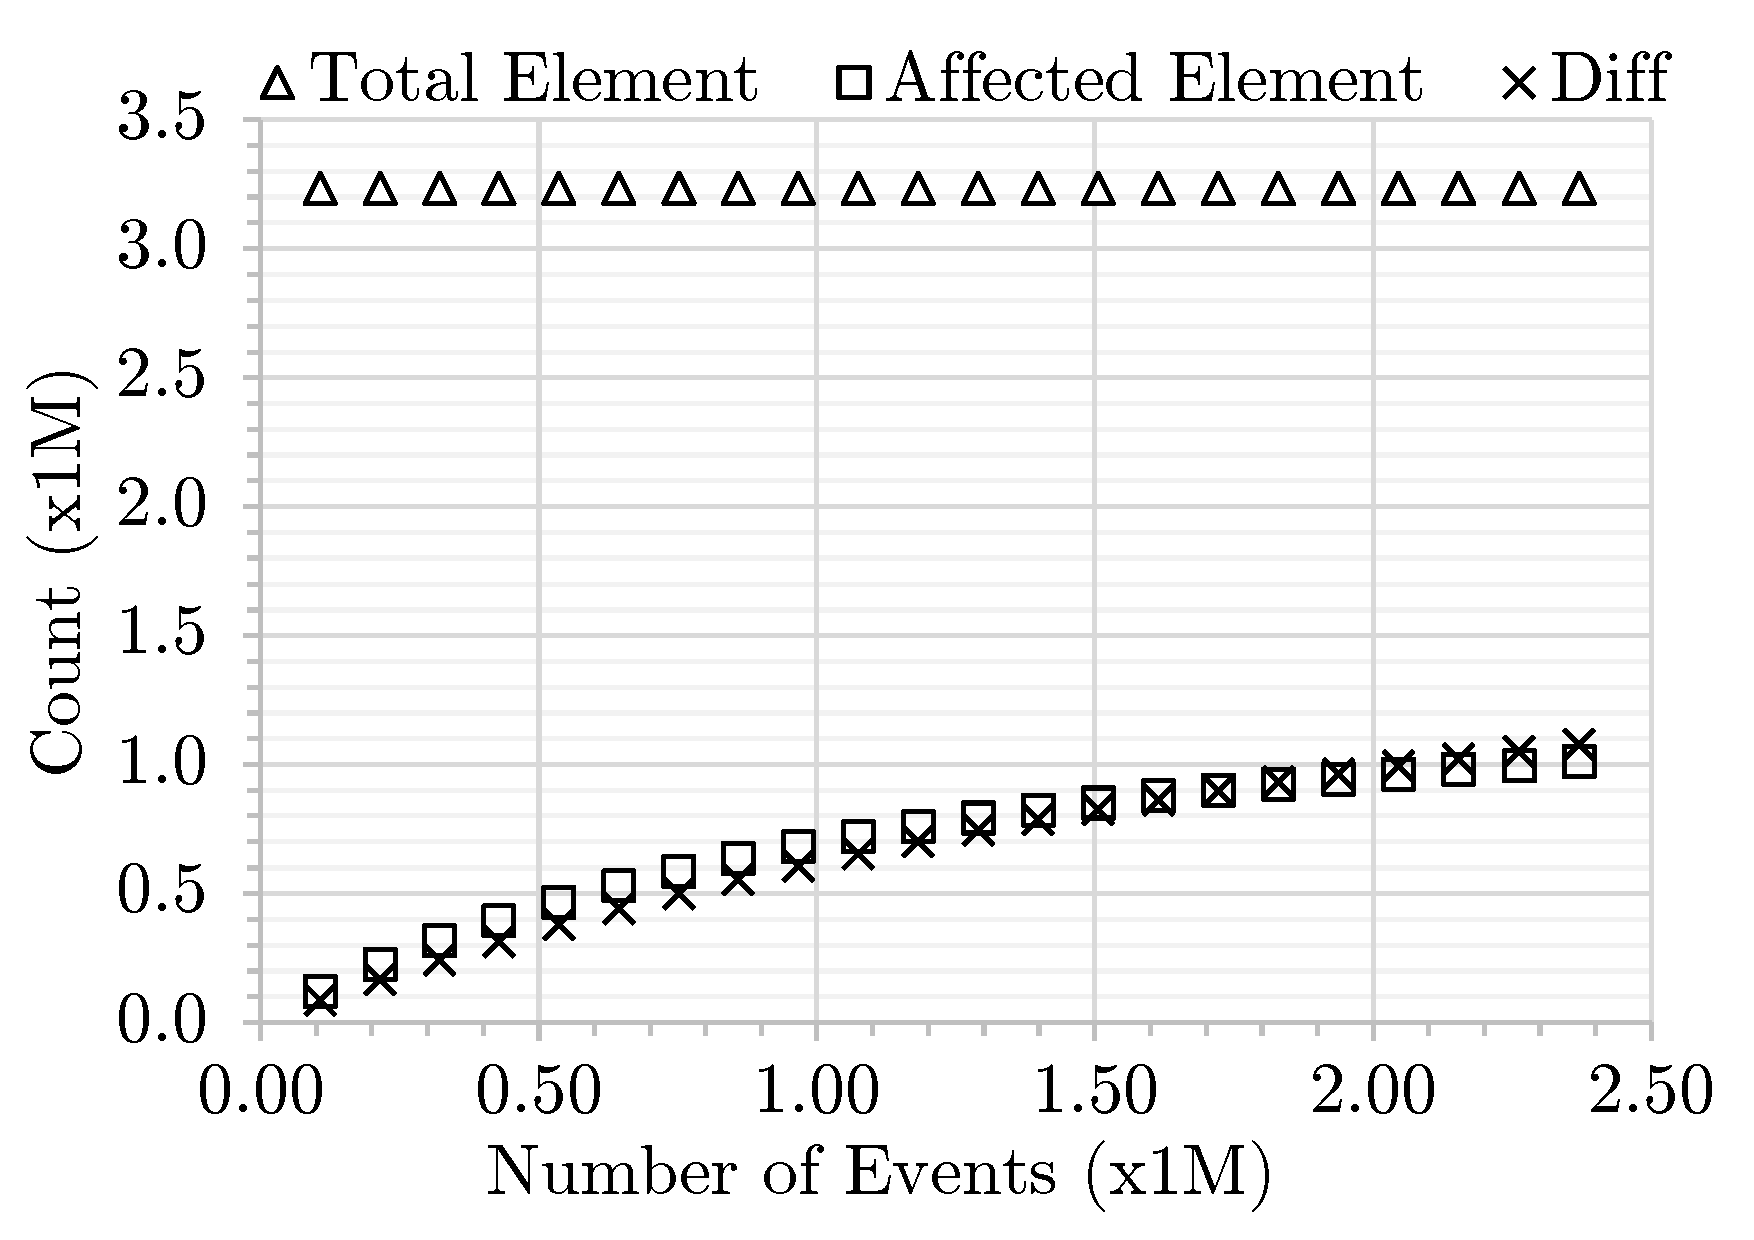
\includegraphics[width=\linewidth]{mixed-count-events}
  \caption{total elements, affected elements, and diffs}
  \label{fig:modification_course}
\end{wrapfigure}

This section reports on the results for comparison time and memory footprint for the mixed and homogeneous operation experiments.

\vspace{-5pt}
\subsubsection{Mixed Operations}
\label{sec:mixed-operation}
In the mixed operation measurement, we modify two identical models differently by applying random operations. As the number of change events generated by the modification grows, the numbers of affected elements and differences also increase in a logarithmic manner. The patterns are shown in Figure \ref{fig:modification_course}. The growth is logarithmic since the probability that the random operations modify the same elements also increases. Thus, some change events might not add new affected elements and differences. In other words, more events are required to increase the number of affected elements or differences. In Figure \ref{fig:modification_course}, the total number of elements remains largely unchanged because the probabilities of addition and deletion were made equal, as noted in Section \ref{sec:evaluation_6}. The figure gives us an insight about the characteristics of the modification caused by the random operations in the mixed operation measurement; it helps to explain the implications of the changes on execution time and memory footprints of model differencing.

\begin{figure}[ht]
  \begin{subfigure}[t]{0.495\linewidth}
    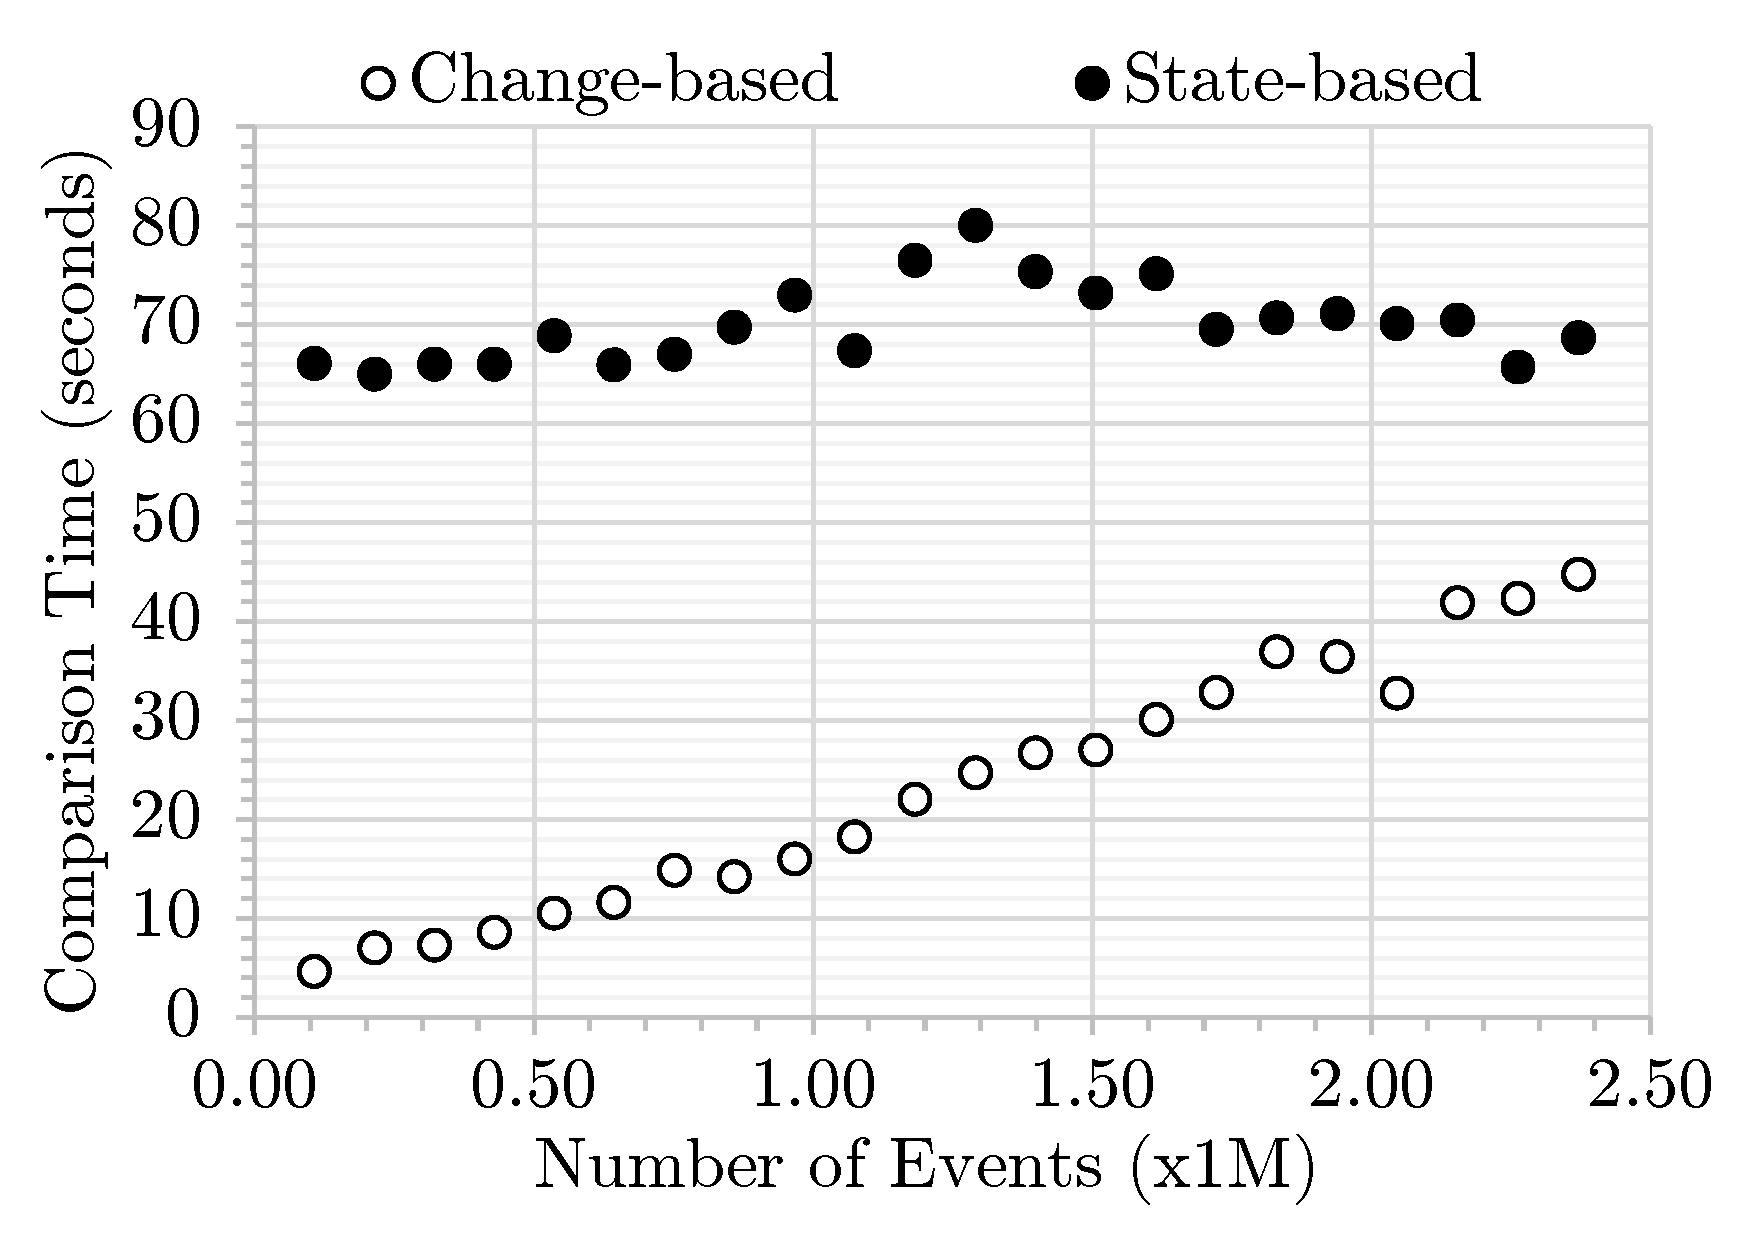
\includegraphics[width=\linewidth]{mixed-time-events}
    \caption{execution time}
    \label{fig:time_diffs}
  \end{subfigure}
  \begin{subfigure}[t]{0.495\linewidth}
    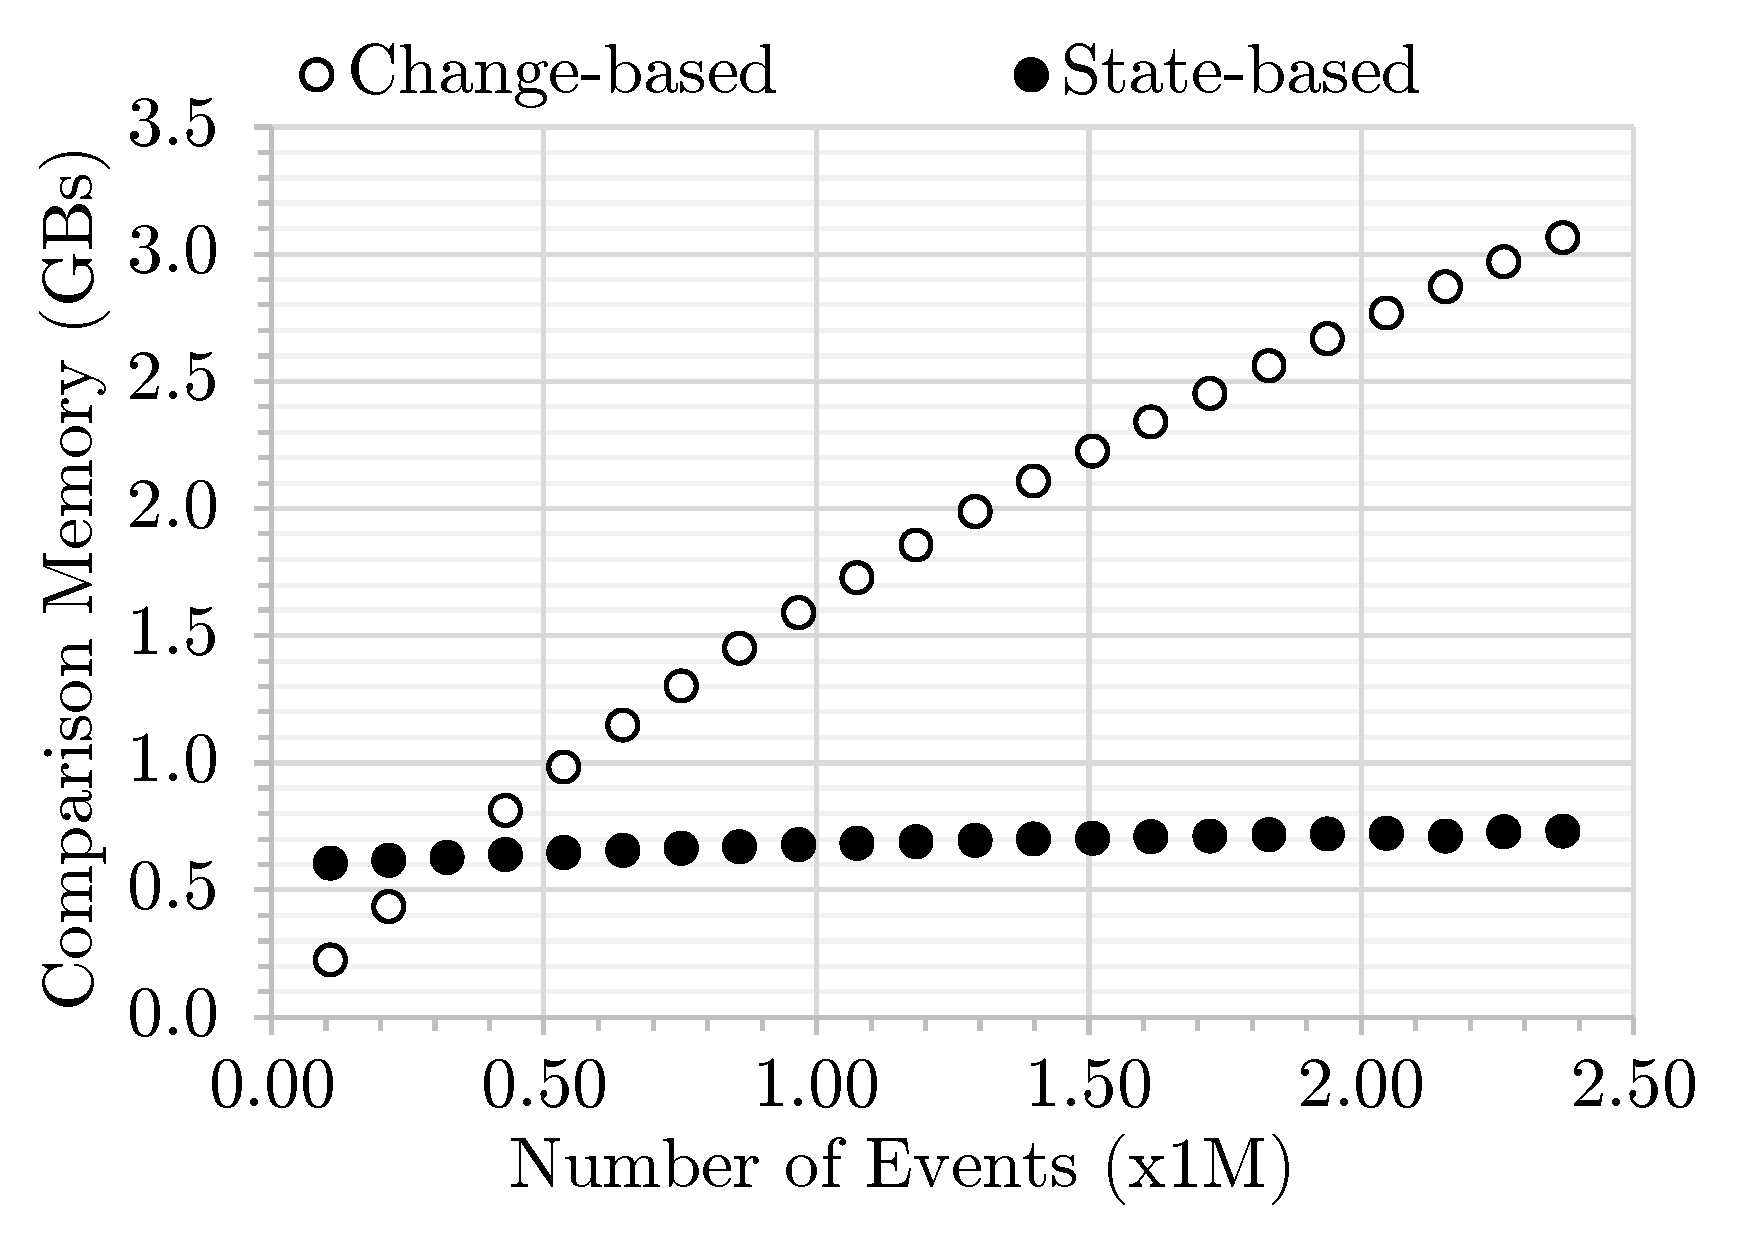
\includegraphics[width=\linewidth]{mixed-memory-events}
    \caption{memory footprint}
    \label{fig:memory_diffs}
  \end{subfigure}
  \caption{Change-based vs. state-based model differencing as differences increase.}
  \label{fig:change_vs_state}
\end{figure}

\begin{figure}[ht]
  \centering
  \begin{subfigure}[t]{0.495\linewidth}
    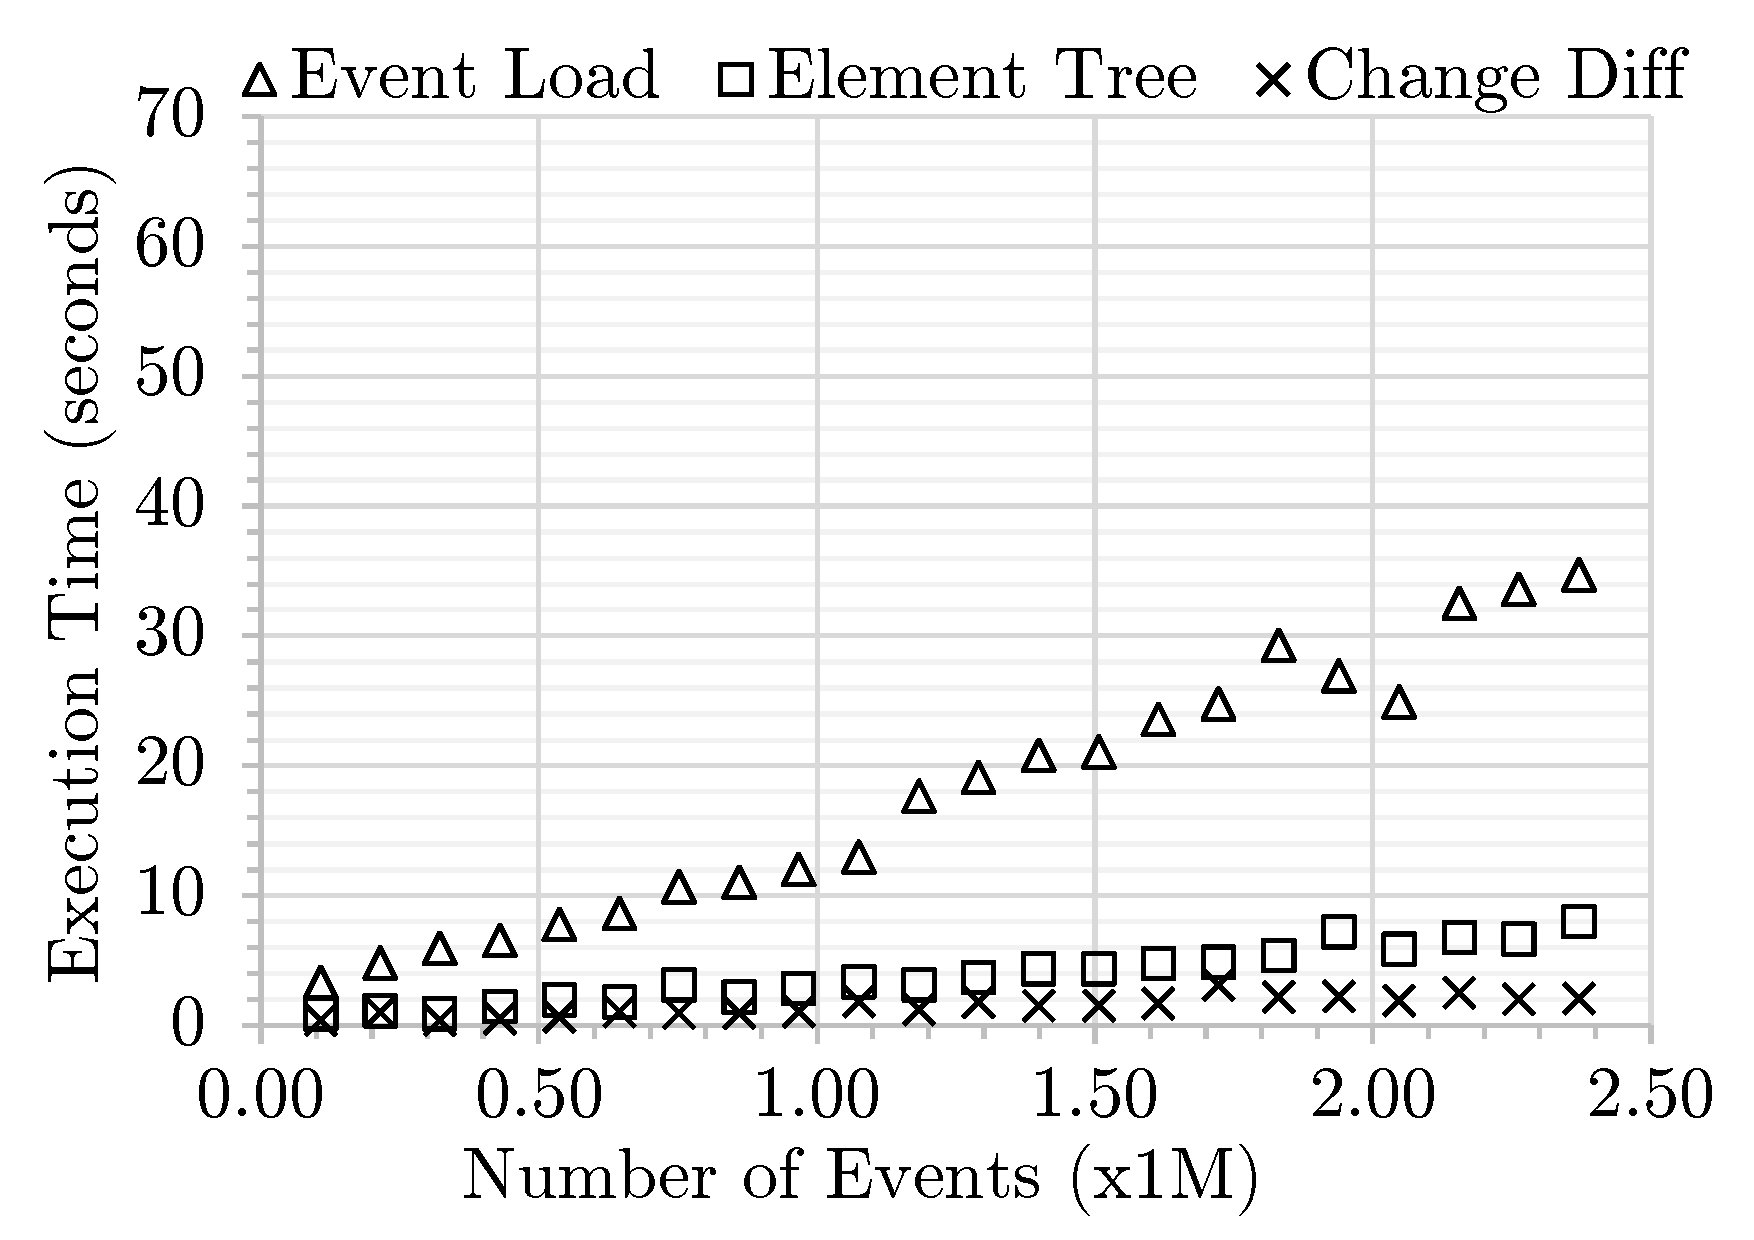
\includegraphics[width=\linewidth]{mixed-time-events-detail}
    \caption{change-based comparison time}
    \label{fig:time_changediff_detail}
  \end{subfigure}
  \hfill
  \begin{subfigure}[t]{0.495\linewidth}
    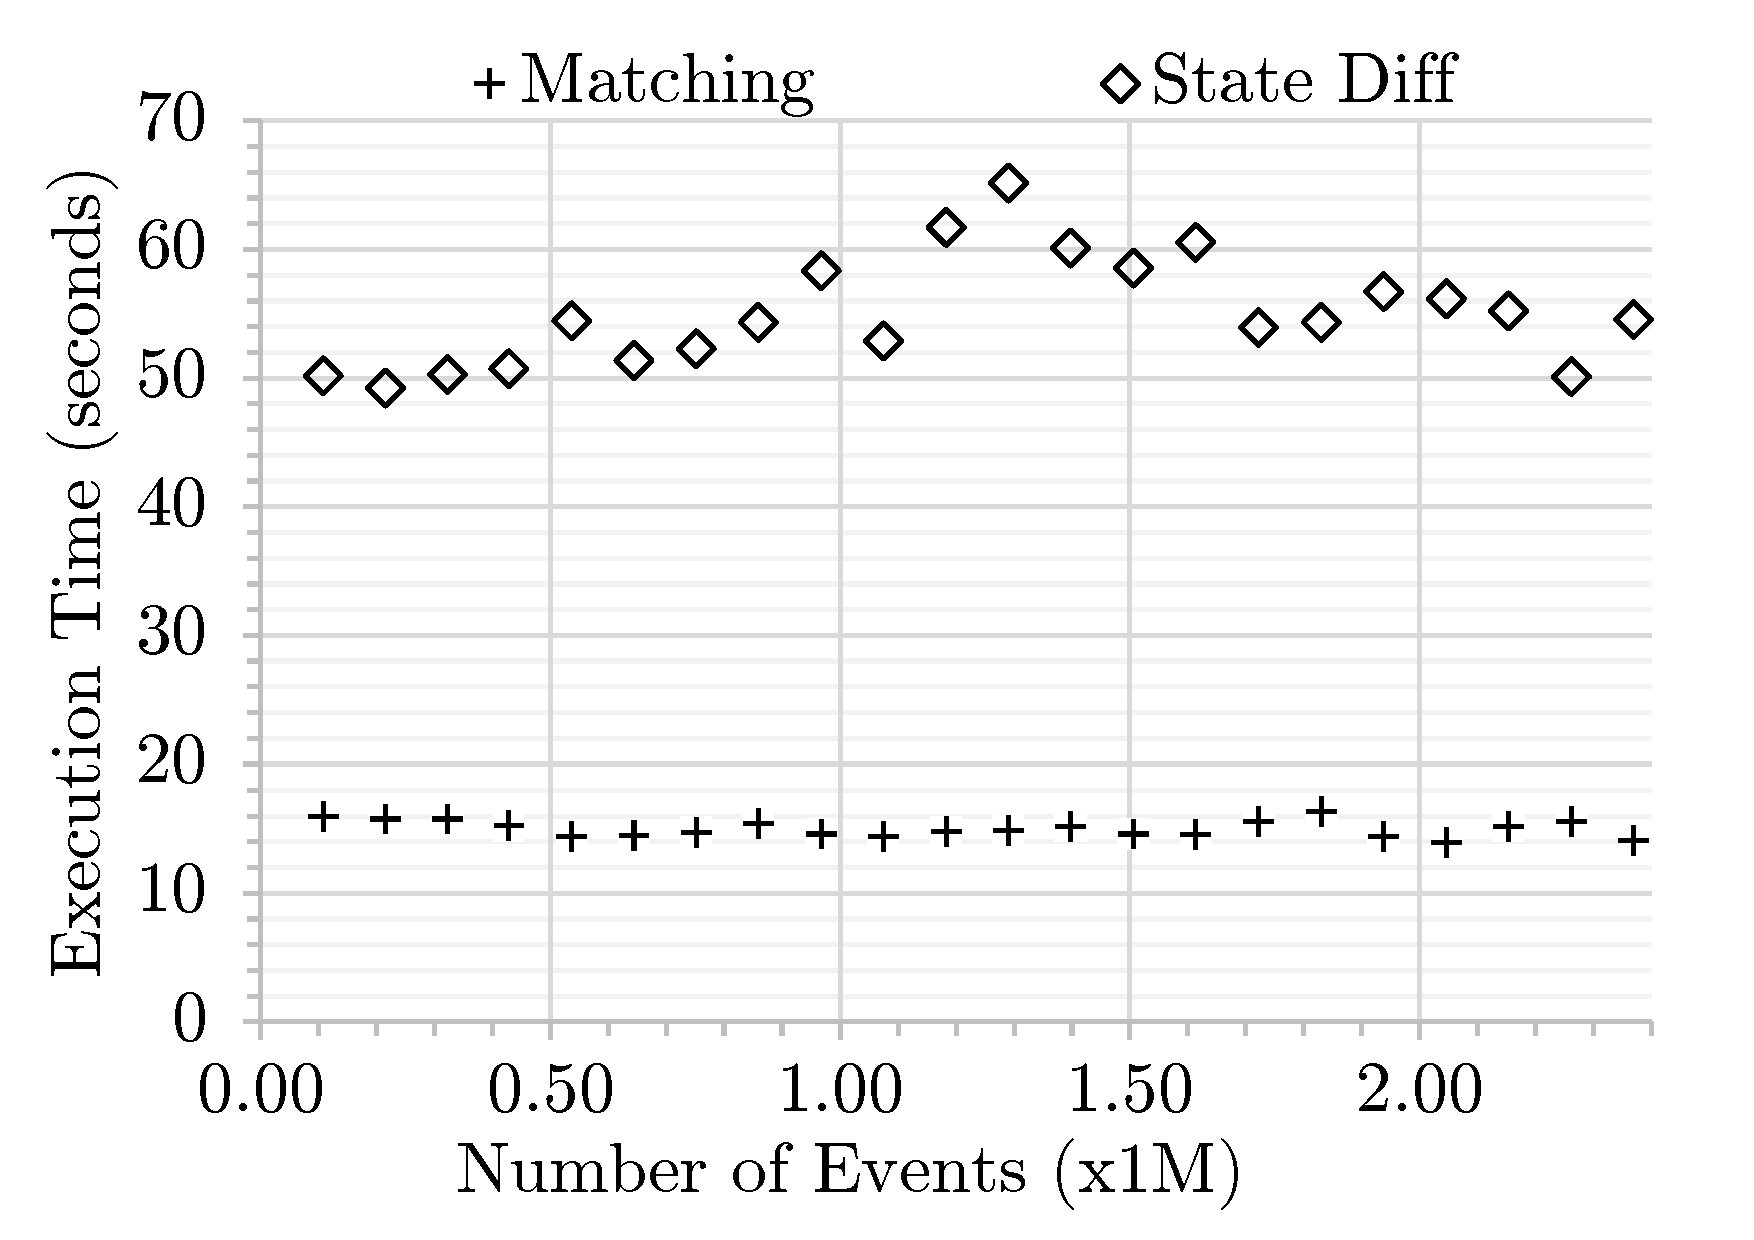
\includegraphics[width=\linewidth]{state-time-events-detail}
    \caption{state-based comparison time}
    \label{fig:time_statediff_detail}
  \end{subfigure}
  \begin{subfigure}[t]{0.495\linewidth}
    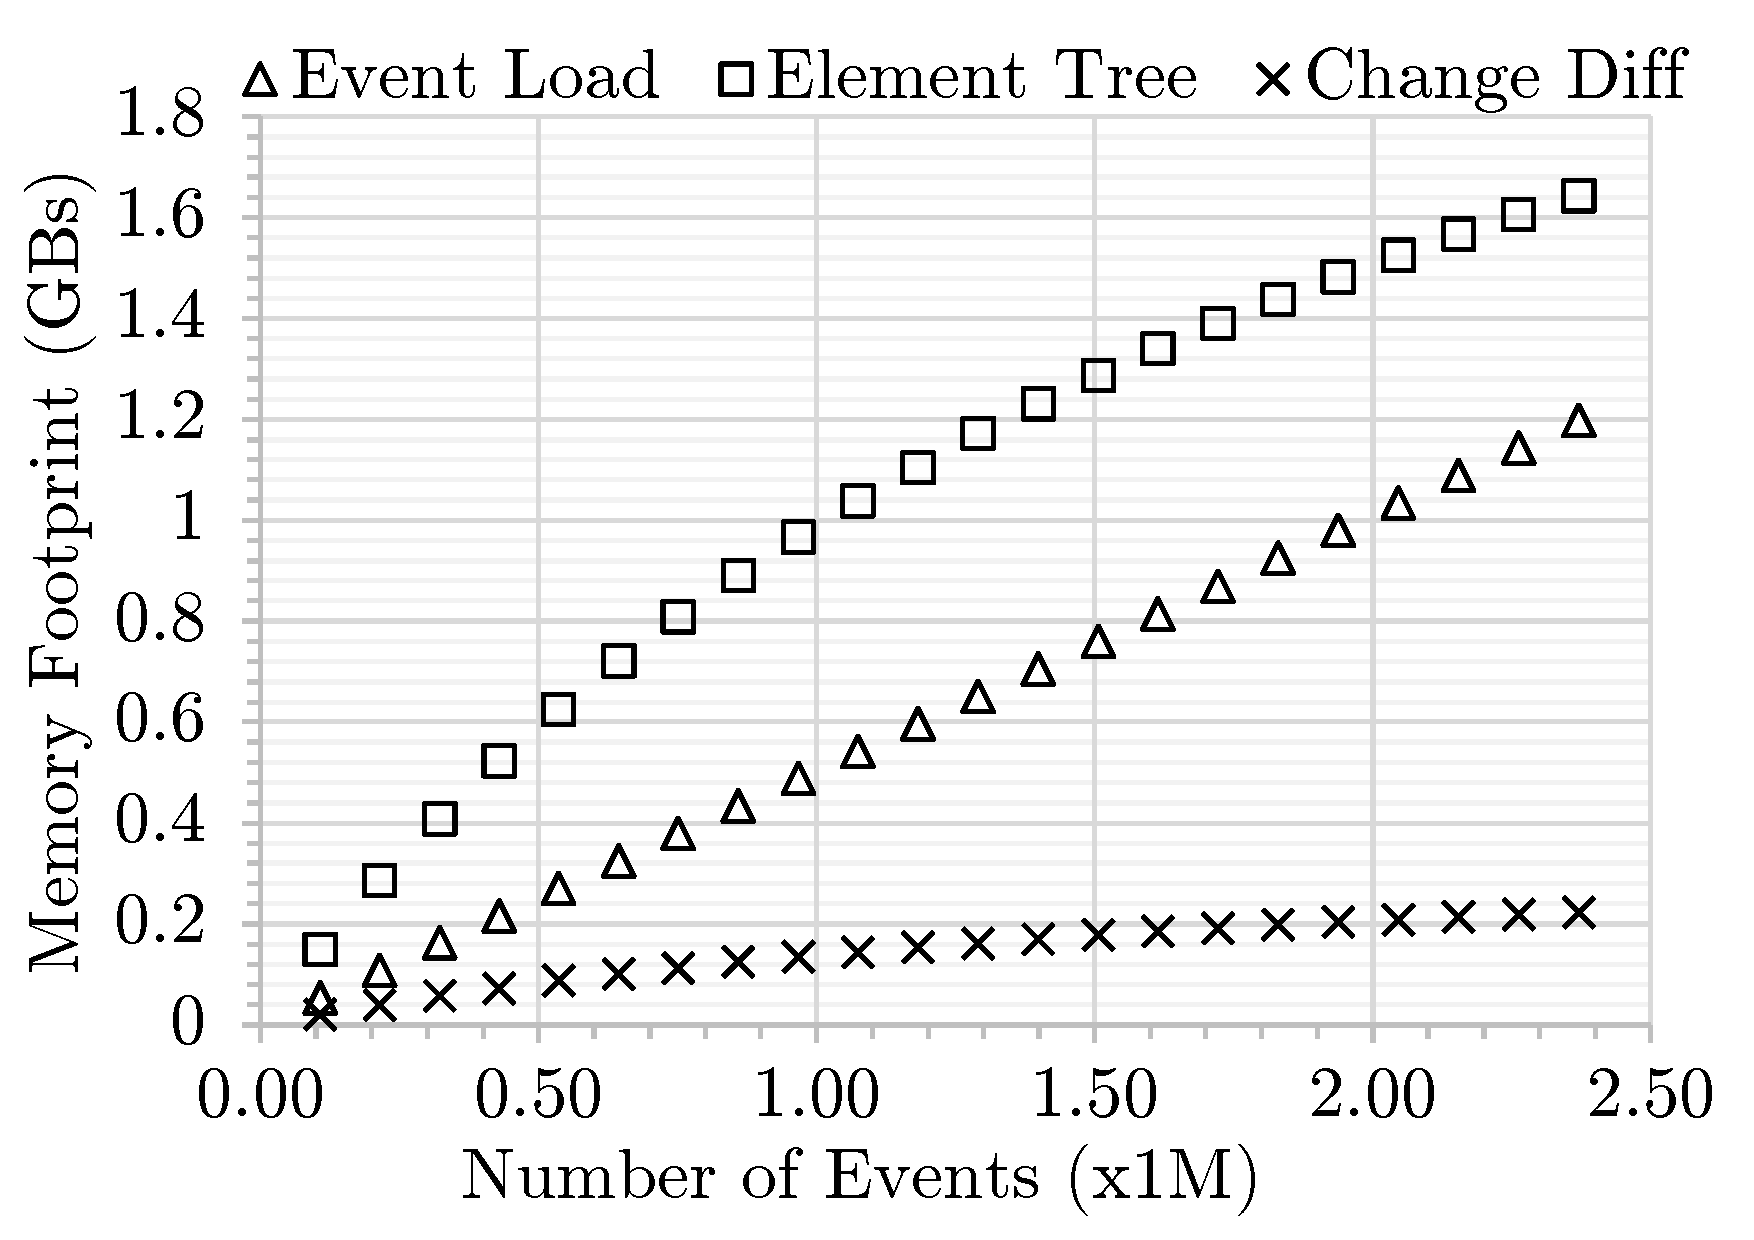
\includegraphics[width=\linewidth]{mixed-memory-events-detail}
    \caption{change-based memory footprint}
    \label{fig:memory_changediff_detail}
  \end{subfigure}
  \hfill
  \begin{subfigure}[t]{0.495\linewidth}
    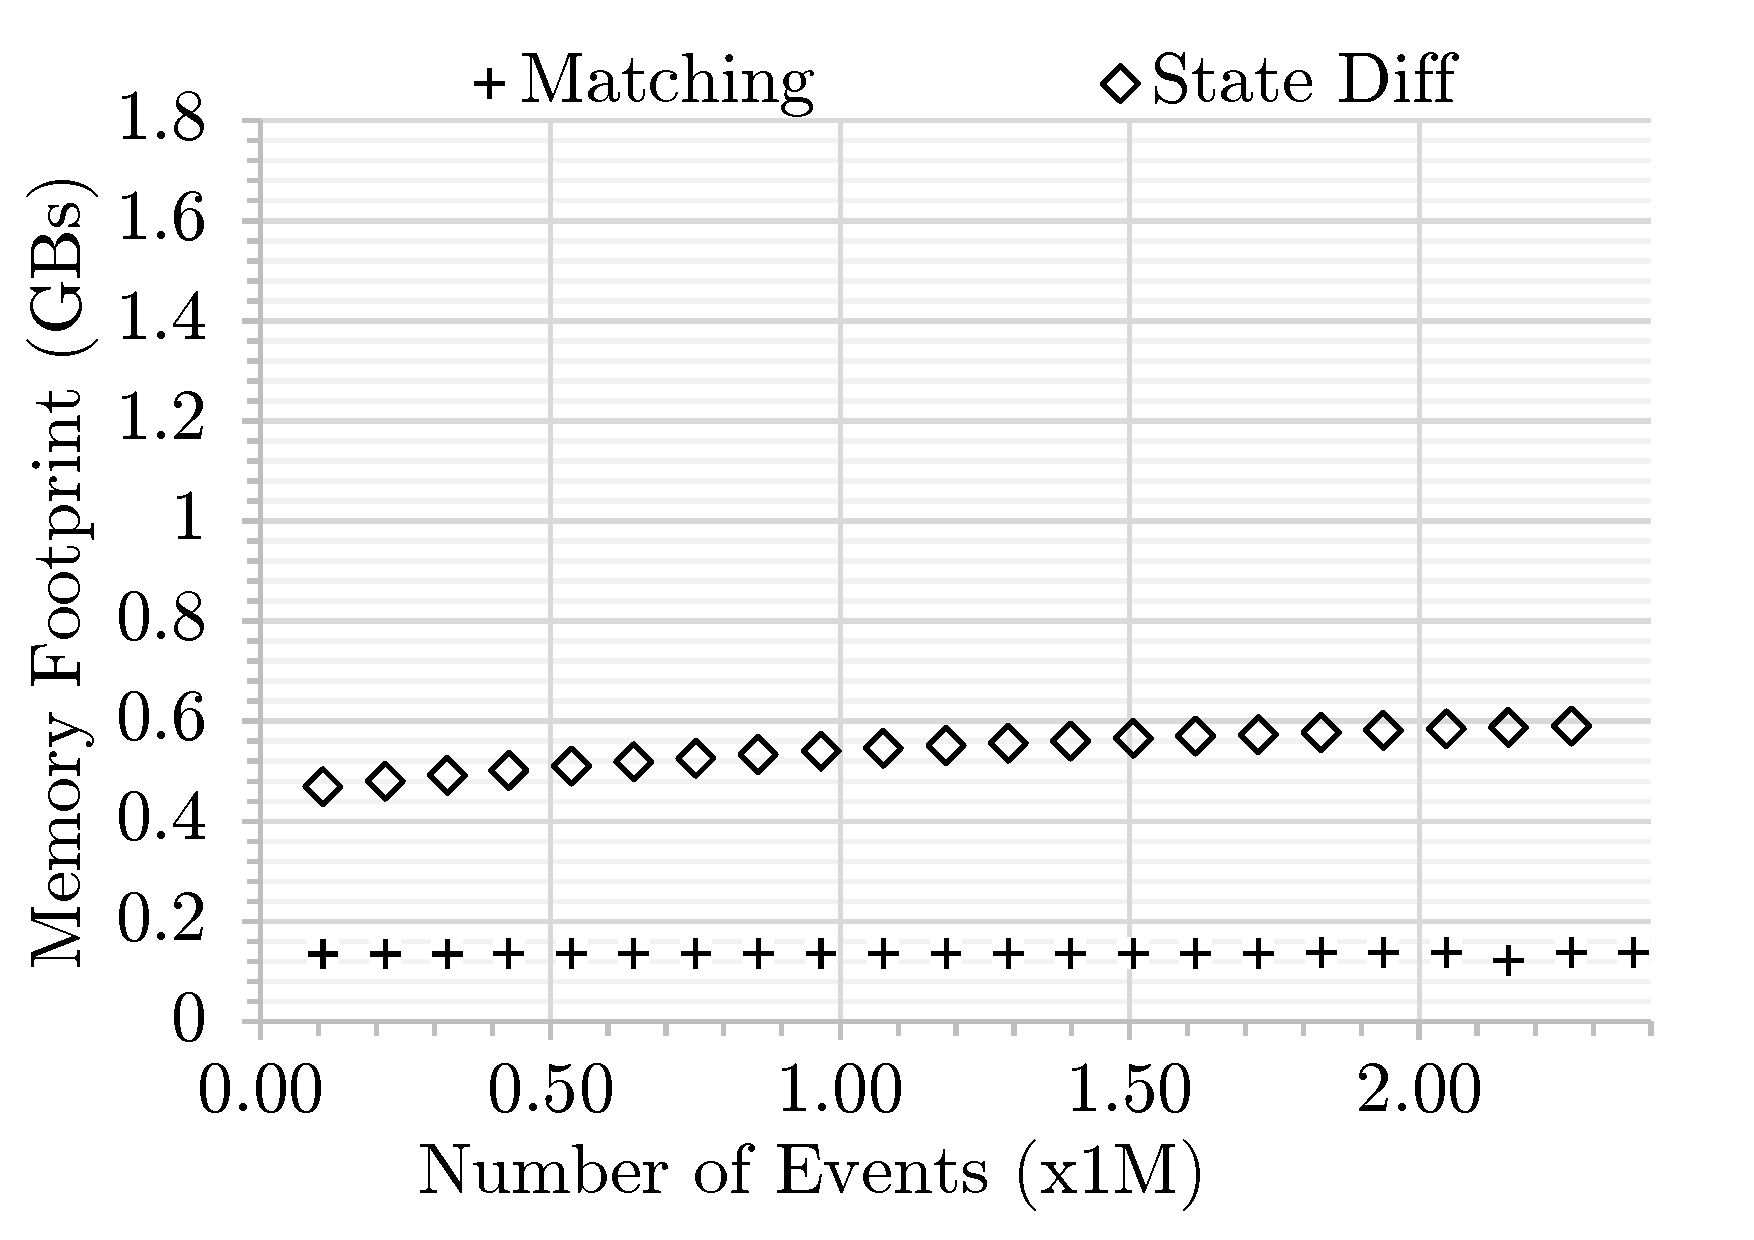
\includegraphics[width=\linewidth]{state-memory-events-detail}
    \caption{state-based memory footprint}
    \label{fig:memory_statediff_detail}
  \end{subfigure}
  \caption{Breakdown view of comparison time and memory footprint in Figure \ref{fig:change_vs_state}.}
  \label{fig:time_memory_detail}
\end{figure}

After applying some random changes on both models, the modification produces 100,000 change events at the first measurement point. Using this amount of events, our change-based comparison takes only 5 seconds to identify around 90,000 differences, in contrast to state-based comparison, which takes 66 seconds (see the first measurement points in Figures \ref{fig:modification_course} and \ref{fig:time_diffs}). If the modification continues, more change events are generated. This growing number of change events must be loaded into memory and thus slows down the change-based comparison. Nevertheless, change-based comparison is still faster than state-based comparison. Even when the number of change events reaches 2.37 million—more than 1 million differences  change-based comparison outperforms state-based comparison in execution time (Figure \ref{fig:time_diffs}). Figure \ref{fig:time_changediff_detail} presents the comparison time in detail. It shows that the event loading time is the dominant contributor to the slowdown compared to the element tree’s construction time and diffing time.

For the state-based comparison in Figure \ref{fig:time_statediff_detail}, the comparison time experiences only a slight increase as the number of identified differences also grows.
%\dk{Change to ‘grows’?}
This slight increase comes mainly from the diffing time, while the matching time tends to be constant because of the very small increase of total elements (Figures \ref{fig:modification_course}).

Nevertheless, a change-based comparison generally consumes more memory than a state-based comparison (see Figure \ref{fig:memory_diffs}). It consumes less memory than its state-based counterpart only when the number of events is fewer than 0.3 million. (At that moment there are fewer than 0.25 million identified differences.) Figure \ref{fig:memory_changediff_detail} separates the memory footprint of the change-based comparison into three factors: the loaded change events, element tree, and diffs. As modification continues, more events are generated. These events must be loaded into memory since they contain the information needed to construct an element tree. The amount of space to keep these change events in memory grows linearly with their number.

In contrast, the memory used for the element tree grows logarithmically. As the number of events increases, the probability that events modify already affected elements also increases. Thus, no additional memory allocation is required for the element tree. Moreover, the element tree occupies most of the memory footprint since it mirrors the partial states—elements, features, and values—of the models that are affected by the changes. In our technical implementation, a feature can have many instances—one instance for each element. (As a comparison, in the EMF implementation, there is only one instance for a feature. The feature is used as a key so that different elements can have the same feature that maps to different values simultaneously). This contributes to the large memory footprint used by the element tree. The identified change-based diffs, the third factor, are the smallest factor that contributes to the memory footprint of the change-based comparison.

\begin{figure}[ht]
  \centering
  \begin{subfigure}[t]{0.495\linewidth}
    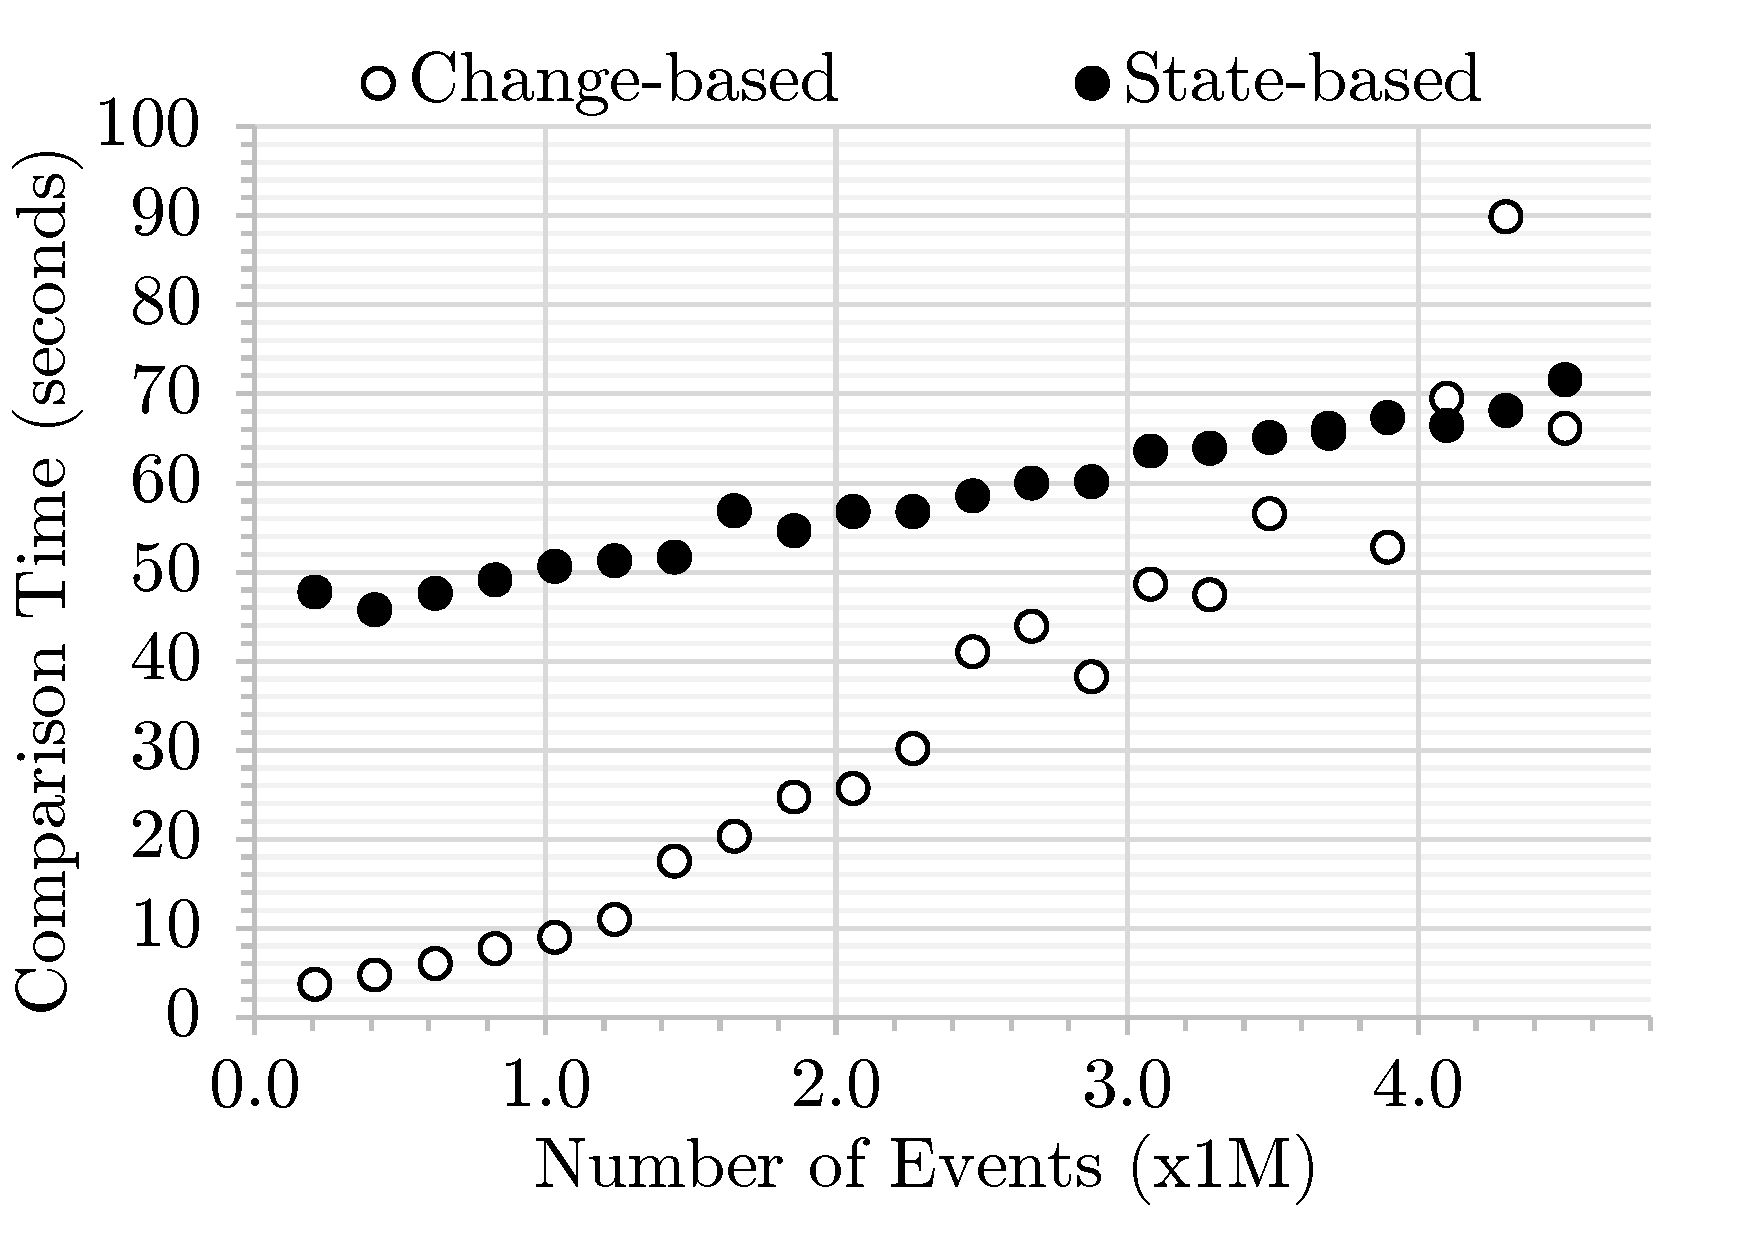
\includegraphics[width=\linewidth]{add-time-events}
    \caption{add-only}
    \label{fig:add-time-events}
  \end{subfigure}
  \hfill
  \begin{subfigure}[t]{0.495\linewidth}
    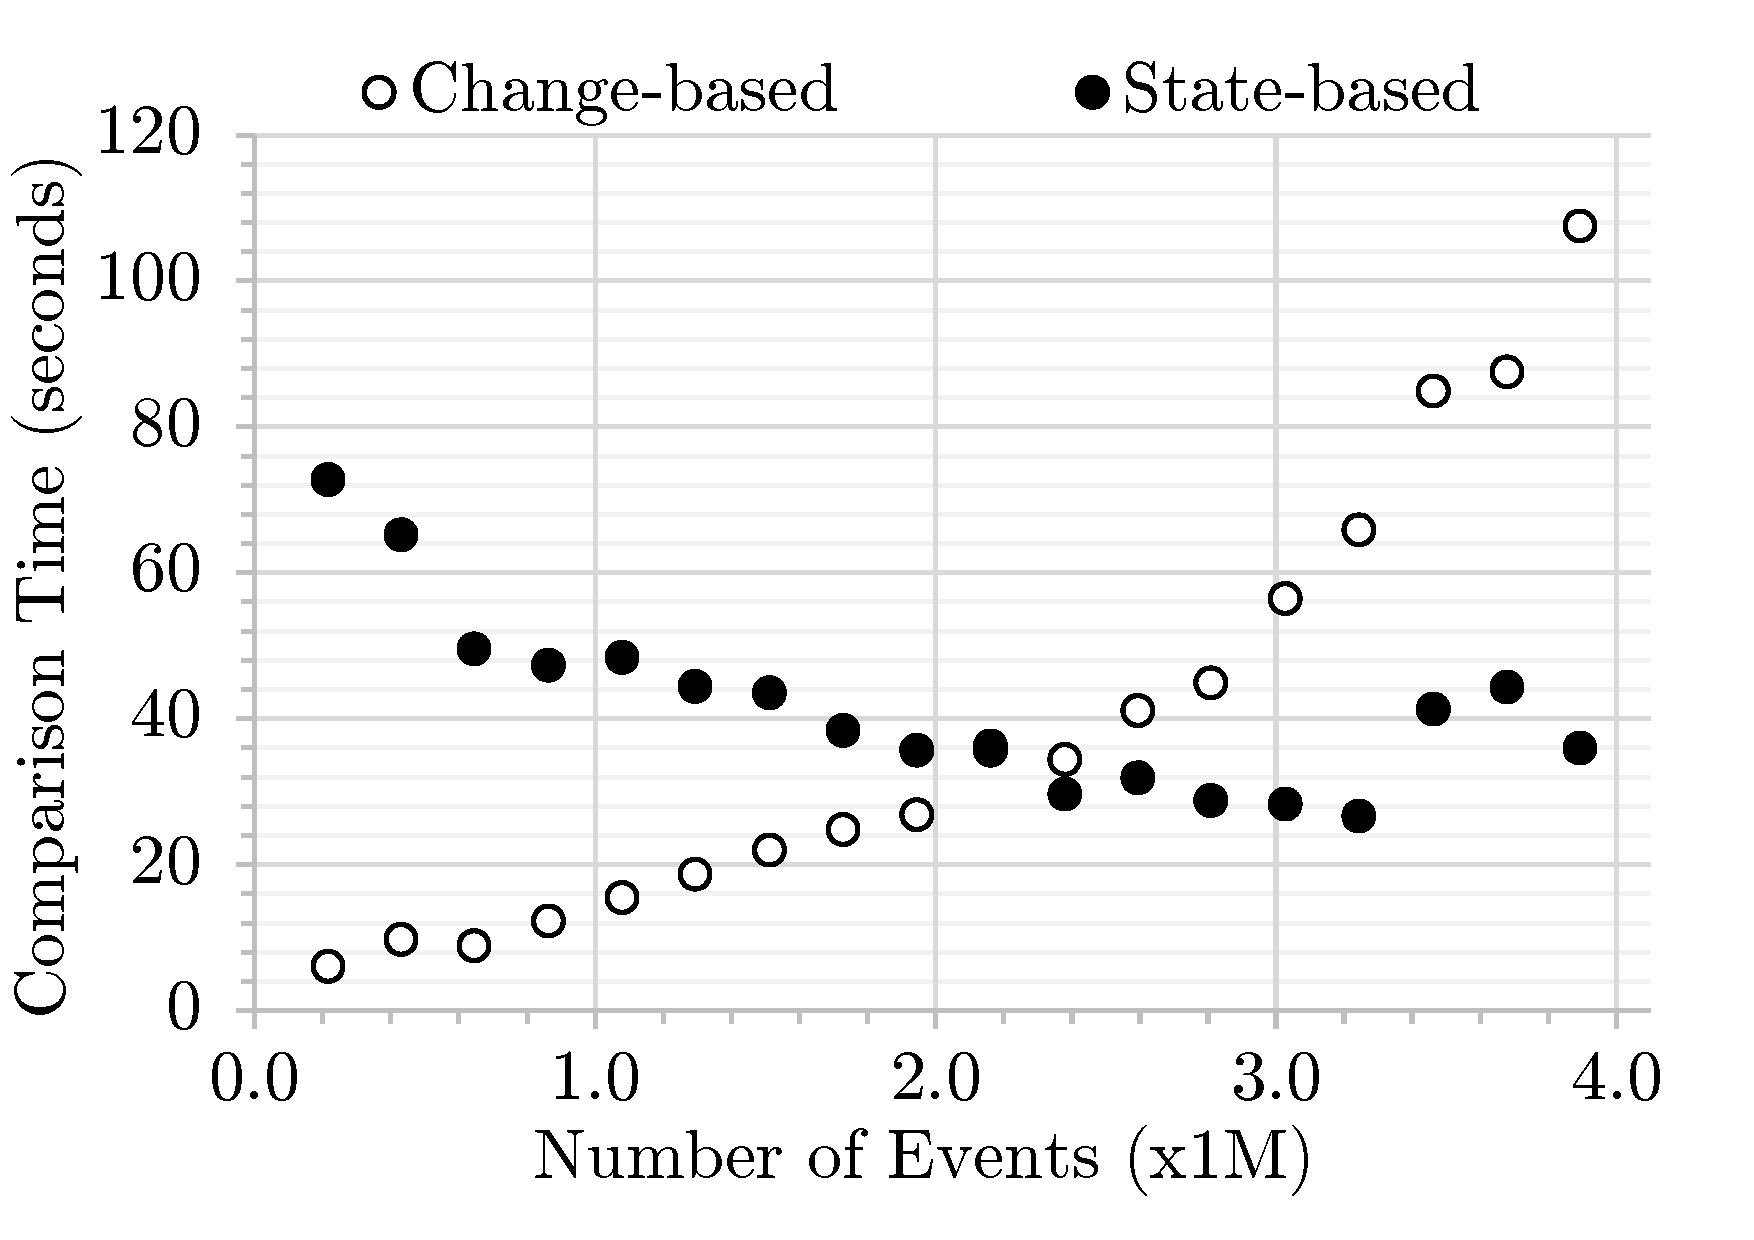
\includegraphics[width=\linewidth]{delete-time-events}
    \caption{delete-only}
    \label{fig:delete-time-events}
  \end{subfigure}
  \begin{subfigure}[t]{0.495\linewidth}
    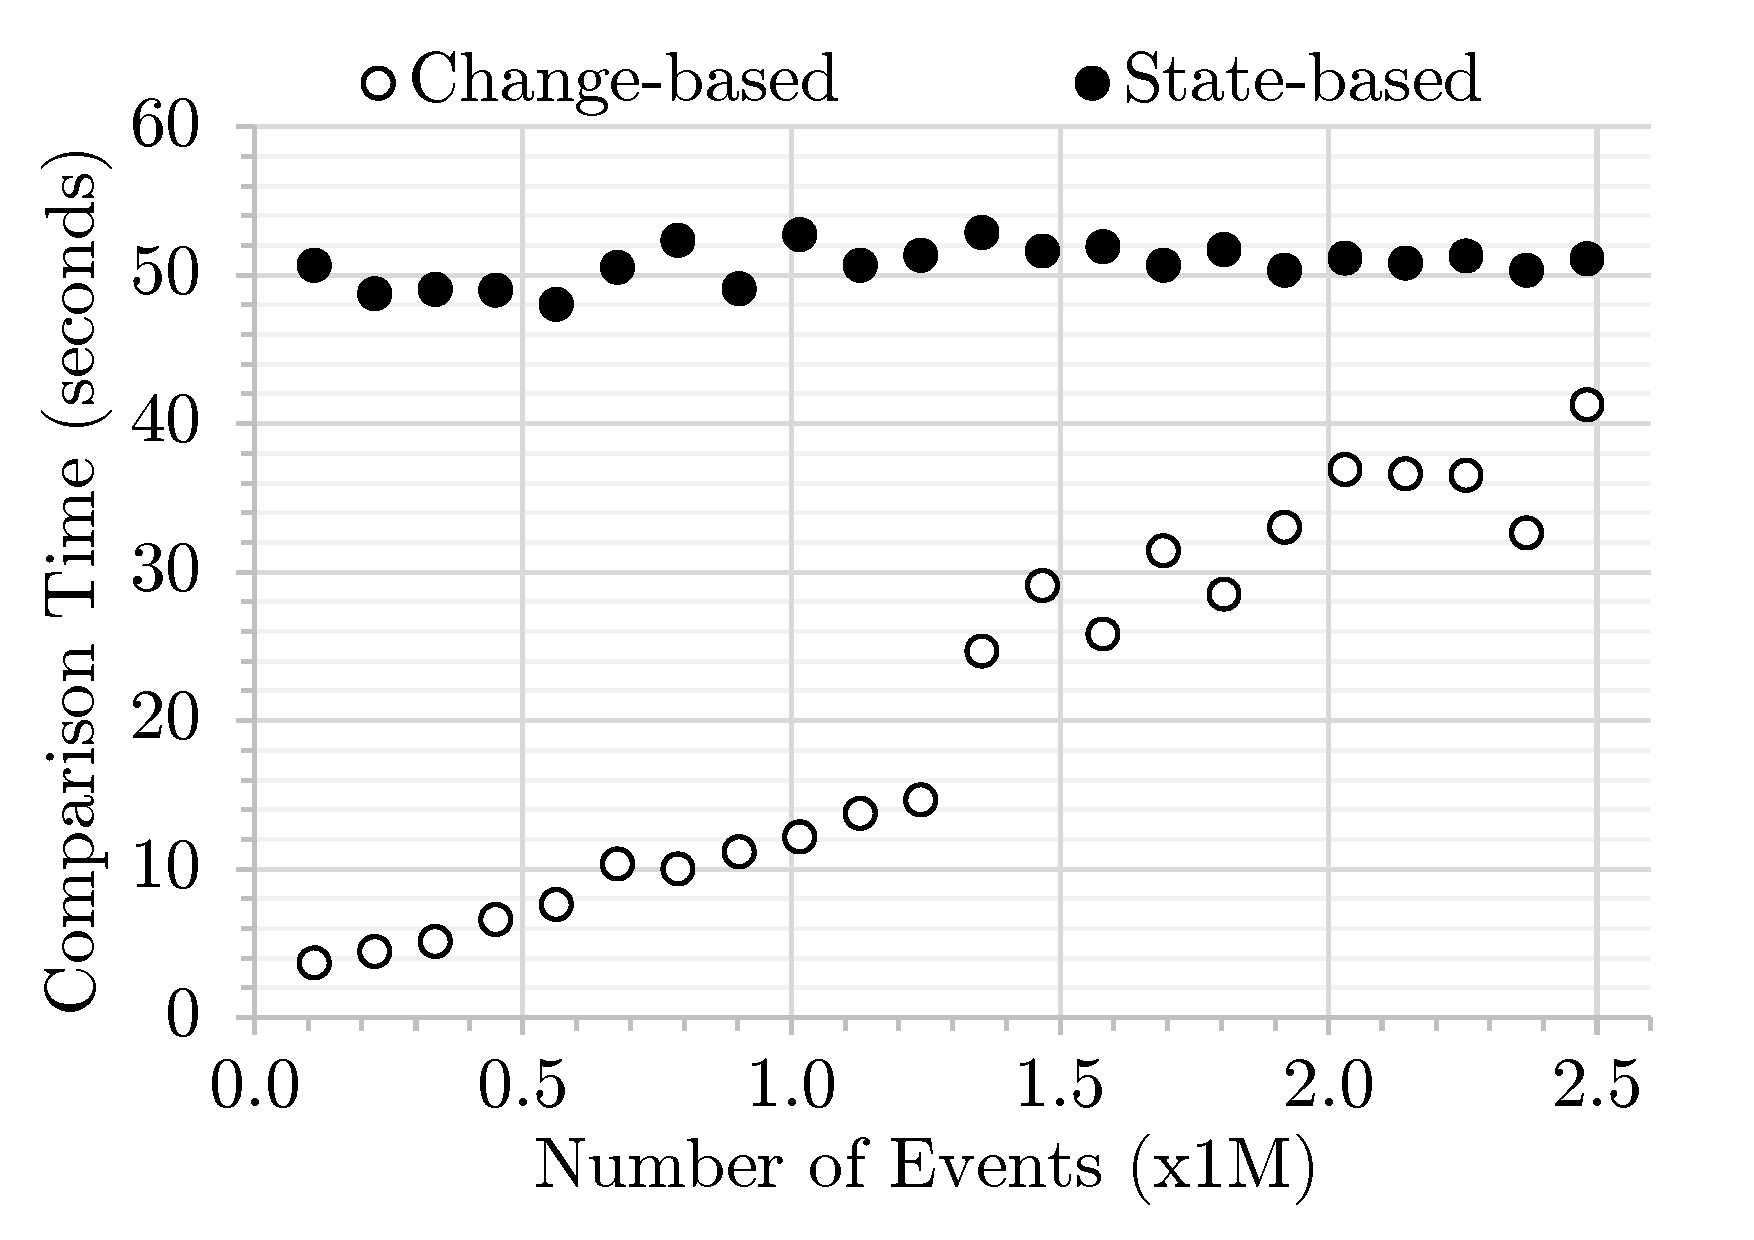
\includegraphics[width=\linewidth]{move-time-events}
    \caption{move-only}
    \label{fig:move-time-events}
  \end{subfigure}
  \hfill
  \begin{subfigure}[t]{0.495\linewidth}
    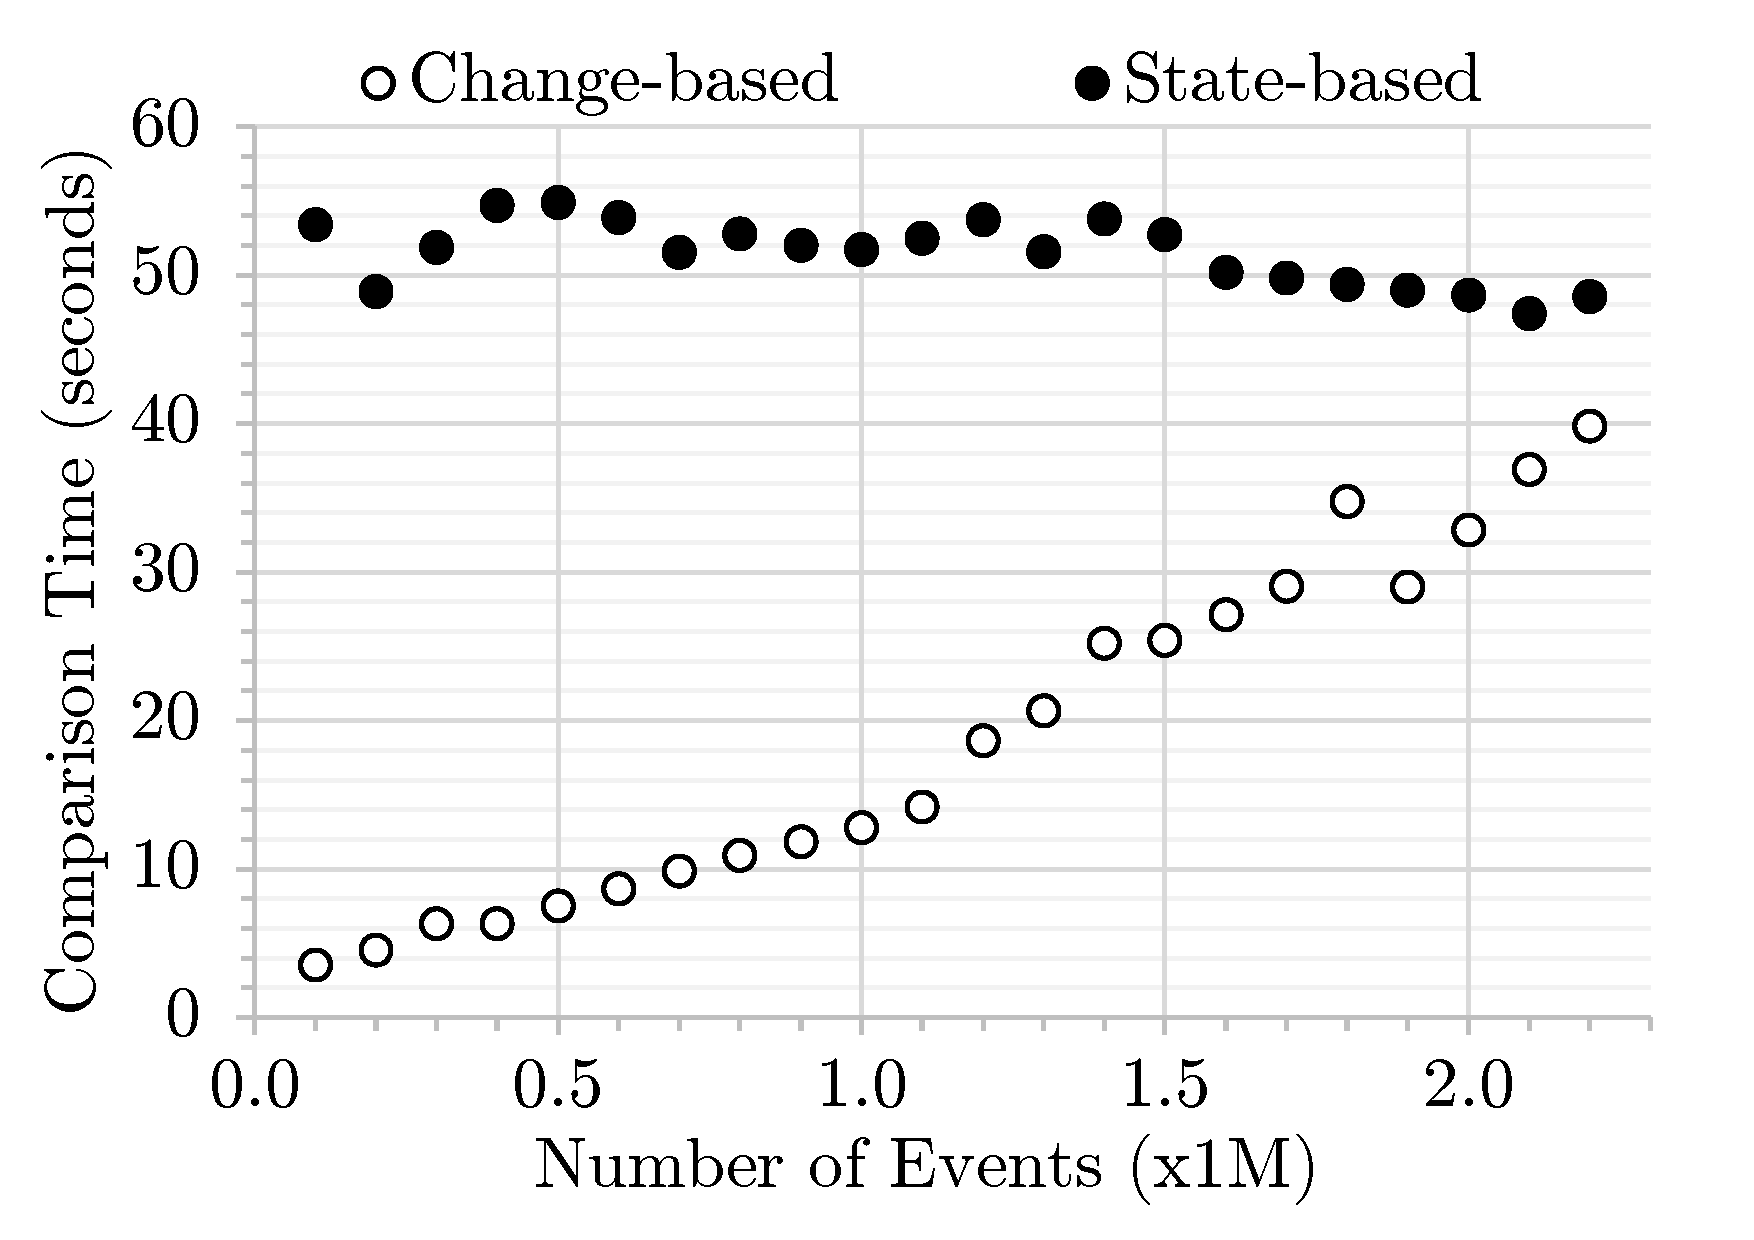
\includegraphics[width=\linewidth]{change-time-events}
    \caption{change-only}
    \label{fig:change-time-events}
  \end{subfigure}
  \caption{Comparison time for homogeneous operations.}
  \label{fig:operation_time_events}
\end{figure}



For the state-based comparison in Figure \ref{fig:memory_statediff_detail}, the memory footprint grows only slightly with the increase of differences. A large part of the memory footprint is used to represent the identified differences, while the memory used for matches tends to be constant, because the changes of the total elements are very few—fewer new elements means less memory must be allocated for new matches (Figures \ref{fig:modification_course}).


\subsubsection{Homogeneous Operations}
\label{sec:homogeneous-operation}

\begin{figure}[ht]
  \centering
  \begin{subfigure}[t]{0.495\linewidth}
    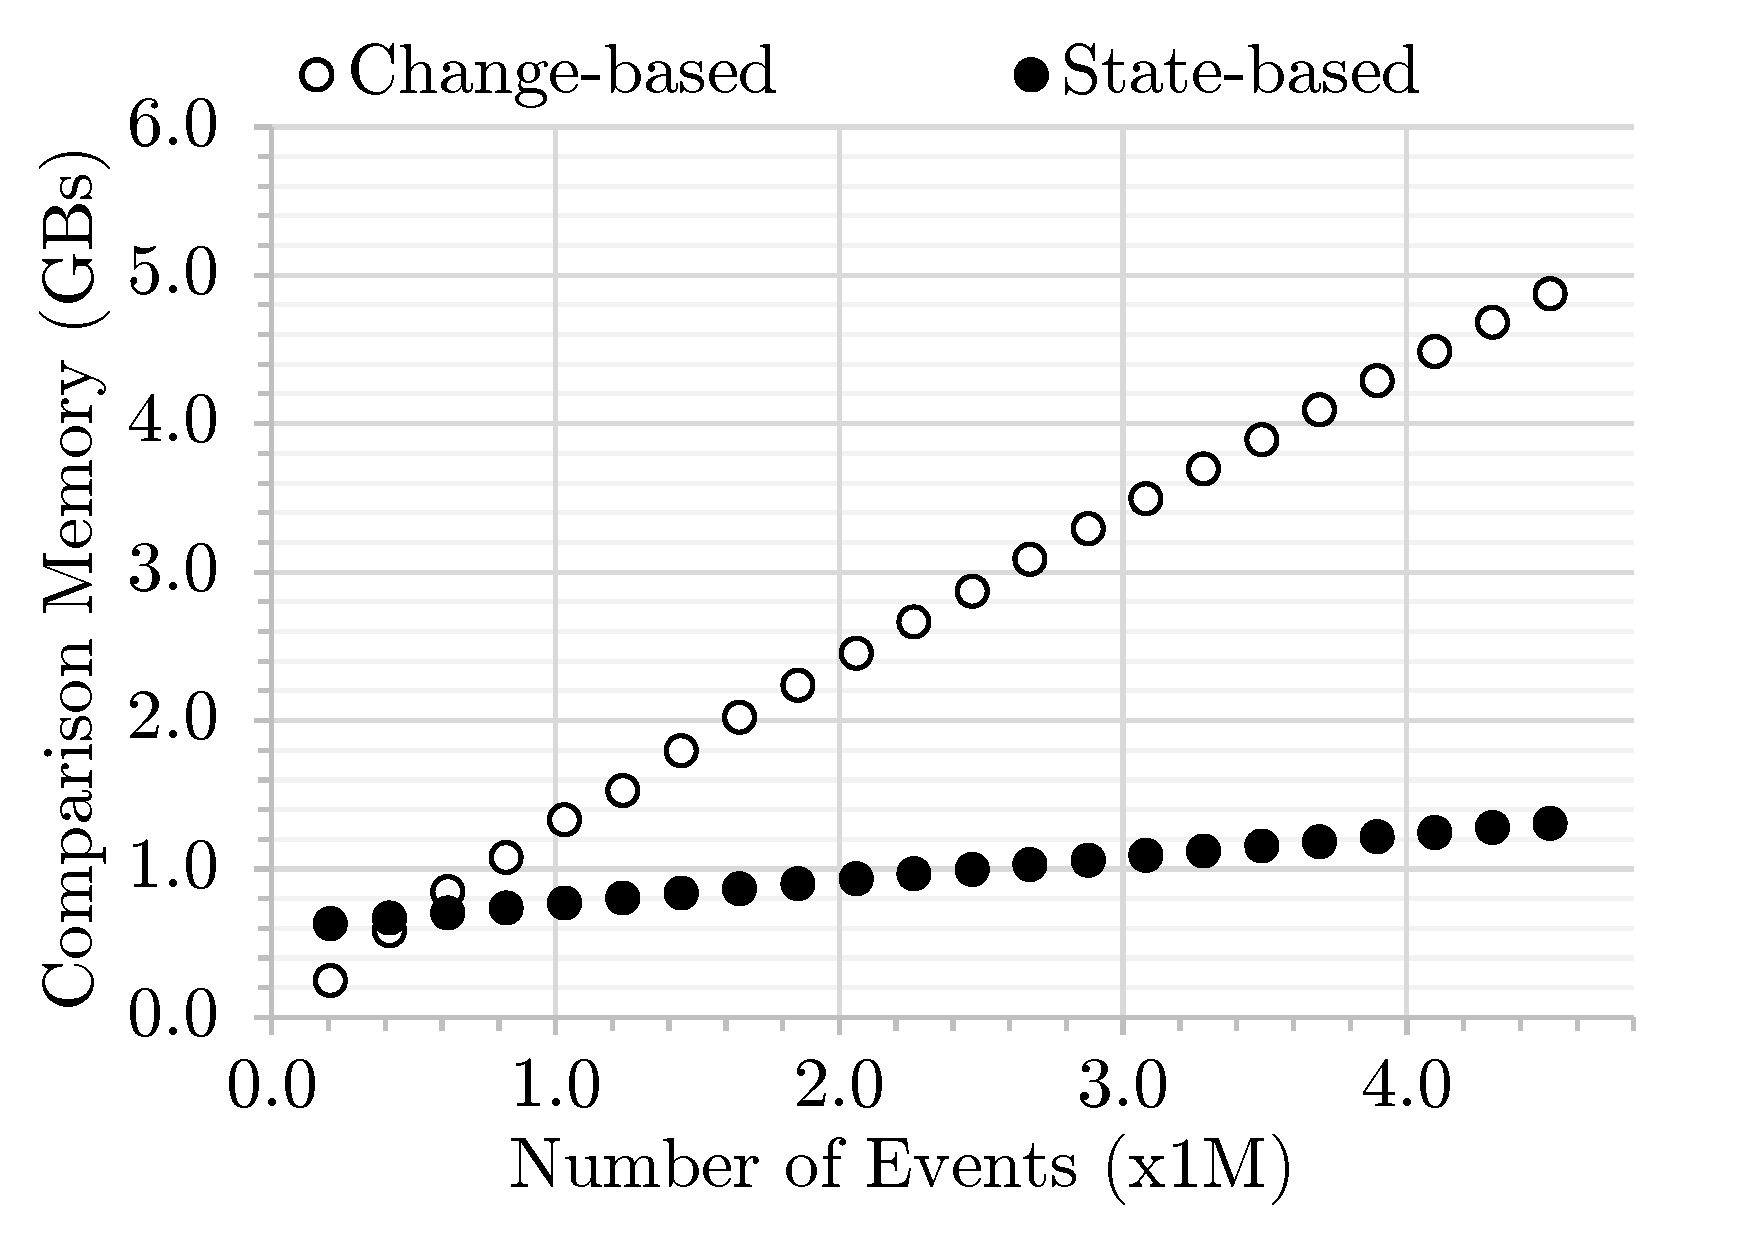
\includegraphics[width=\linewidth]{add-memory-events}
    \caption{add-only}
    \label{fig:add-memory-events}
  \end{subfigure}
  \hfill
  \begin{subfigure}[t]{0.495\linewidth}
    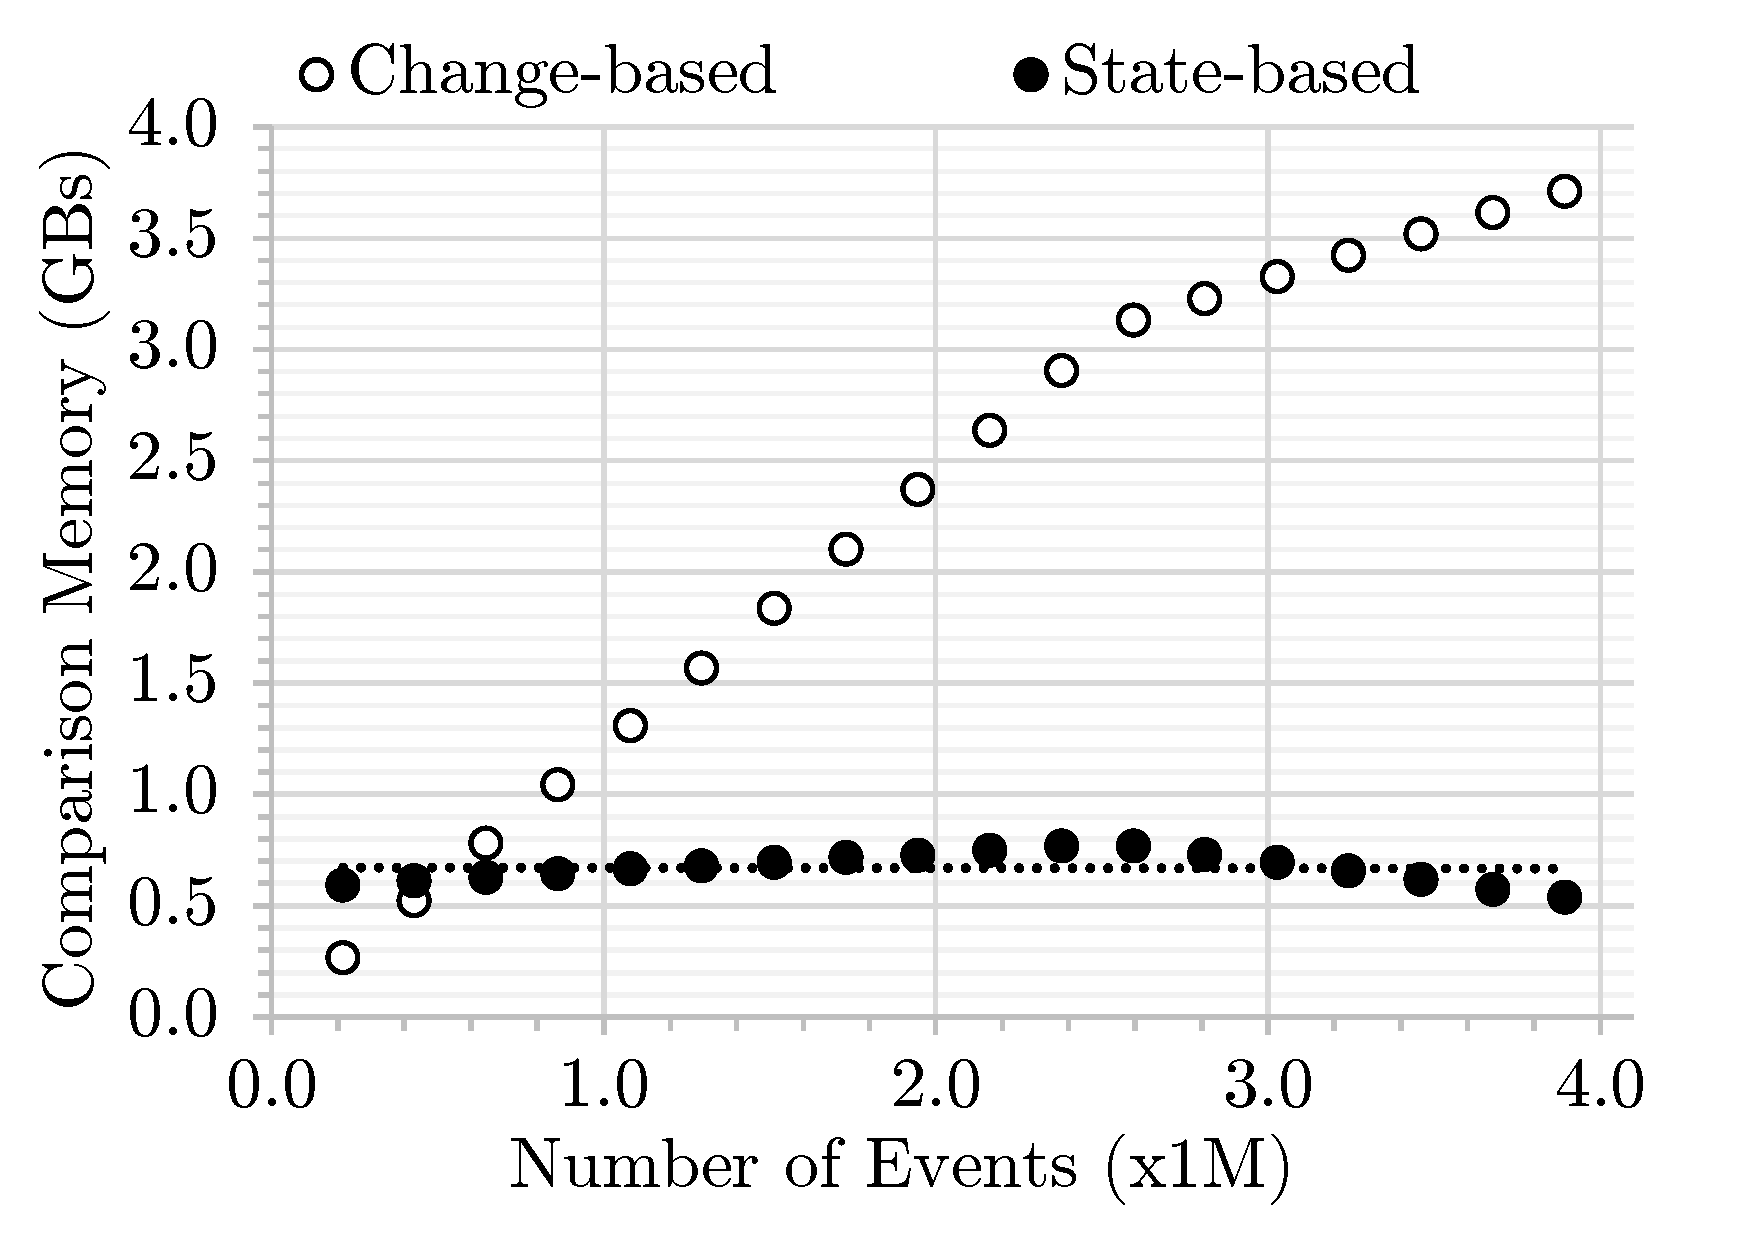
\includegraphics[width=\linewidth]{delete-memory-events}
    \caption{delete-only}
    \label{fig:delete-memory-events}
  \end{subfigure}
  \begin{subfigure}[t]{0.495\linewidth}
    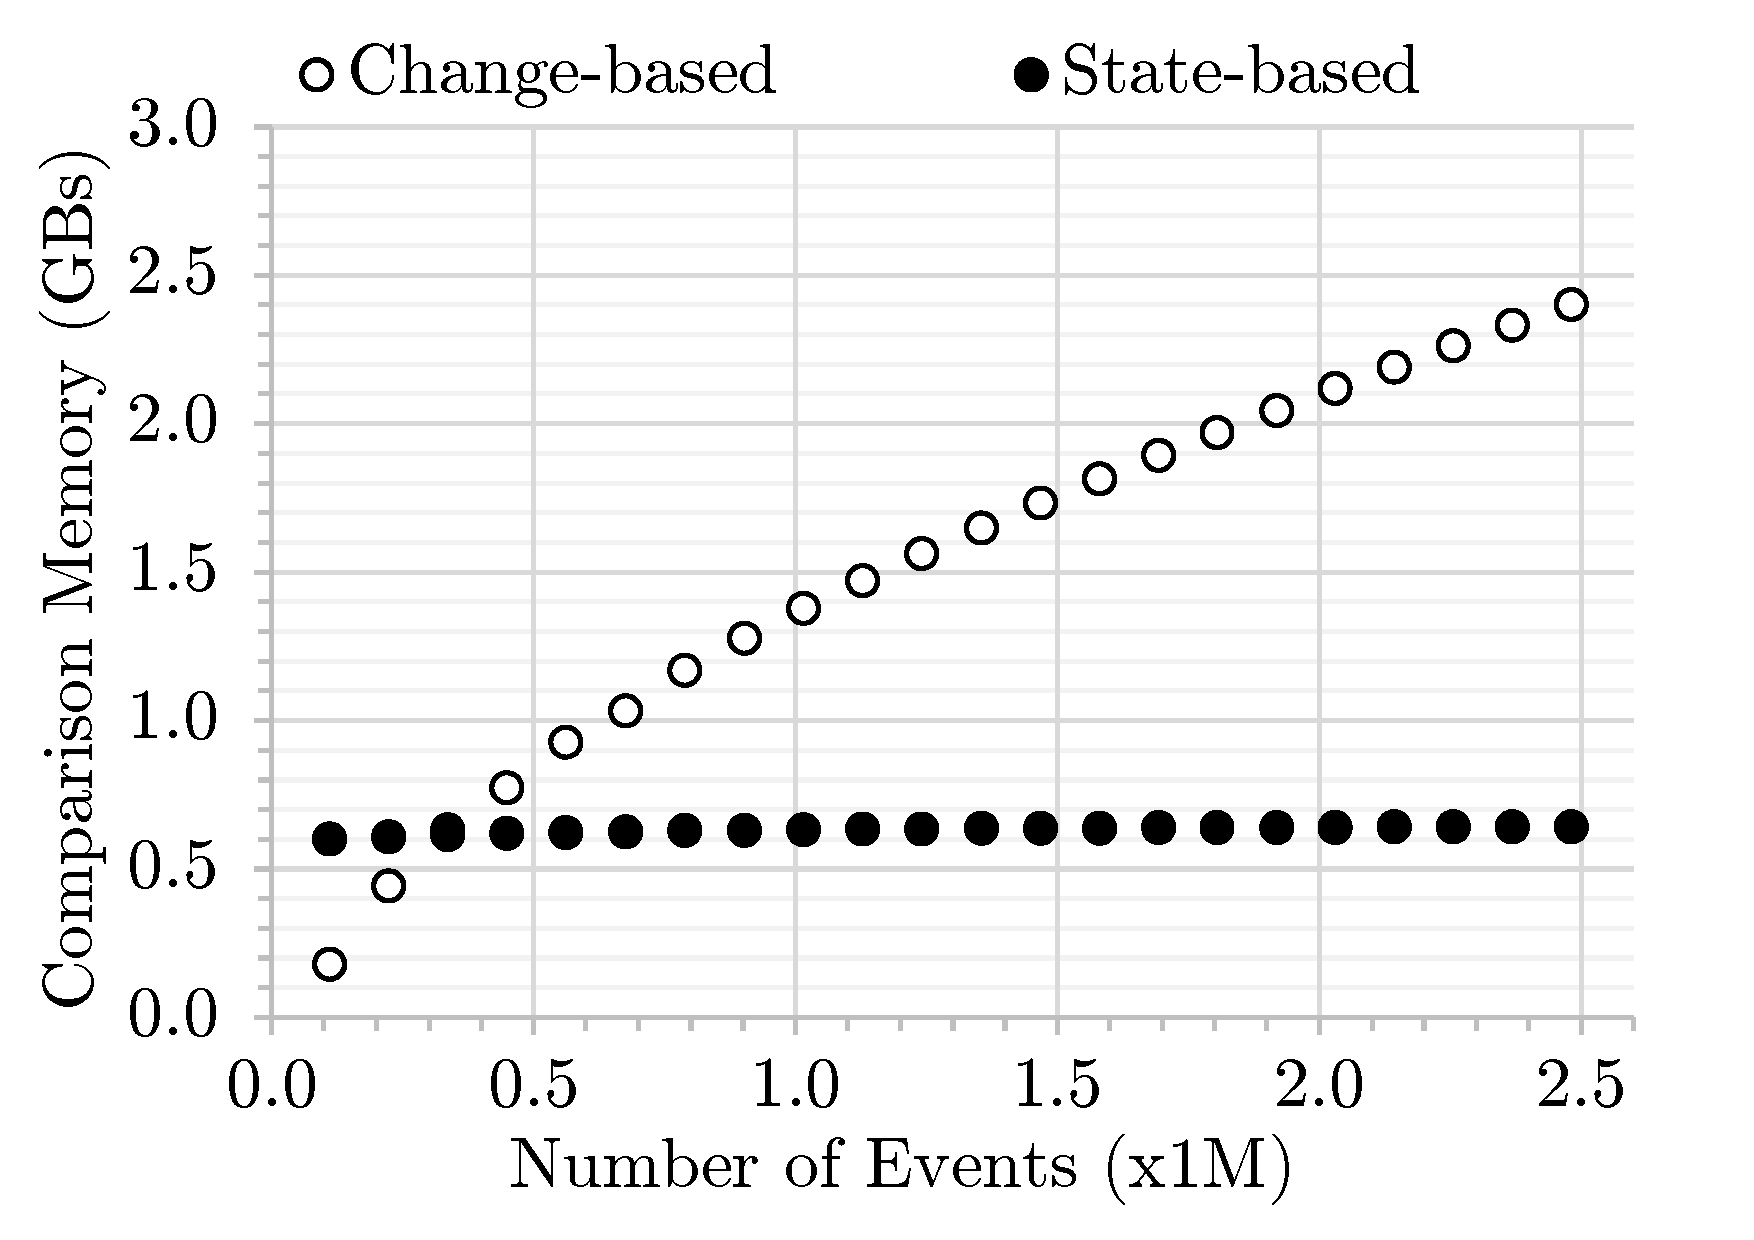
\includegraphics[width=\linewidth]{move-memory-events}
    \caption{move-only}
    \label{fig:move-memory-events}
  \end{subfigure}
  \hfill
  \begin{subfigure}[t]{0.495\linewidth}
    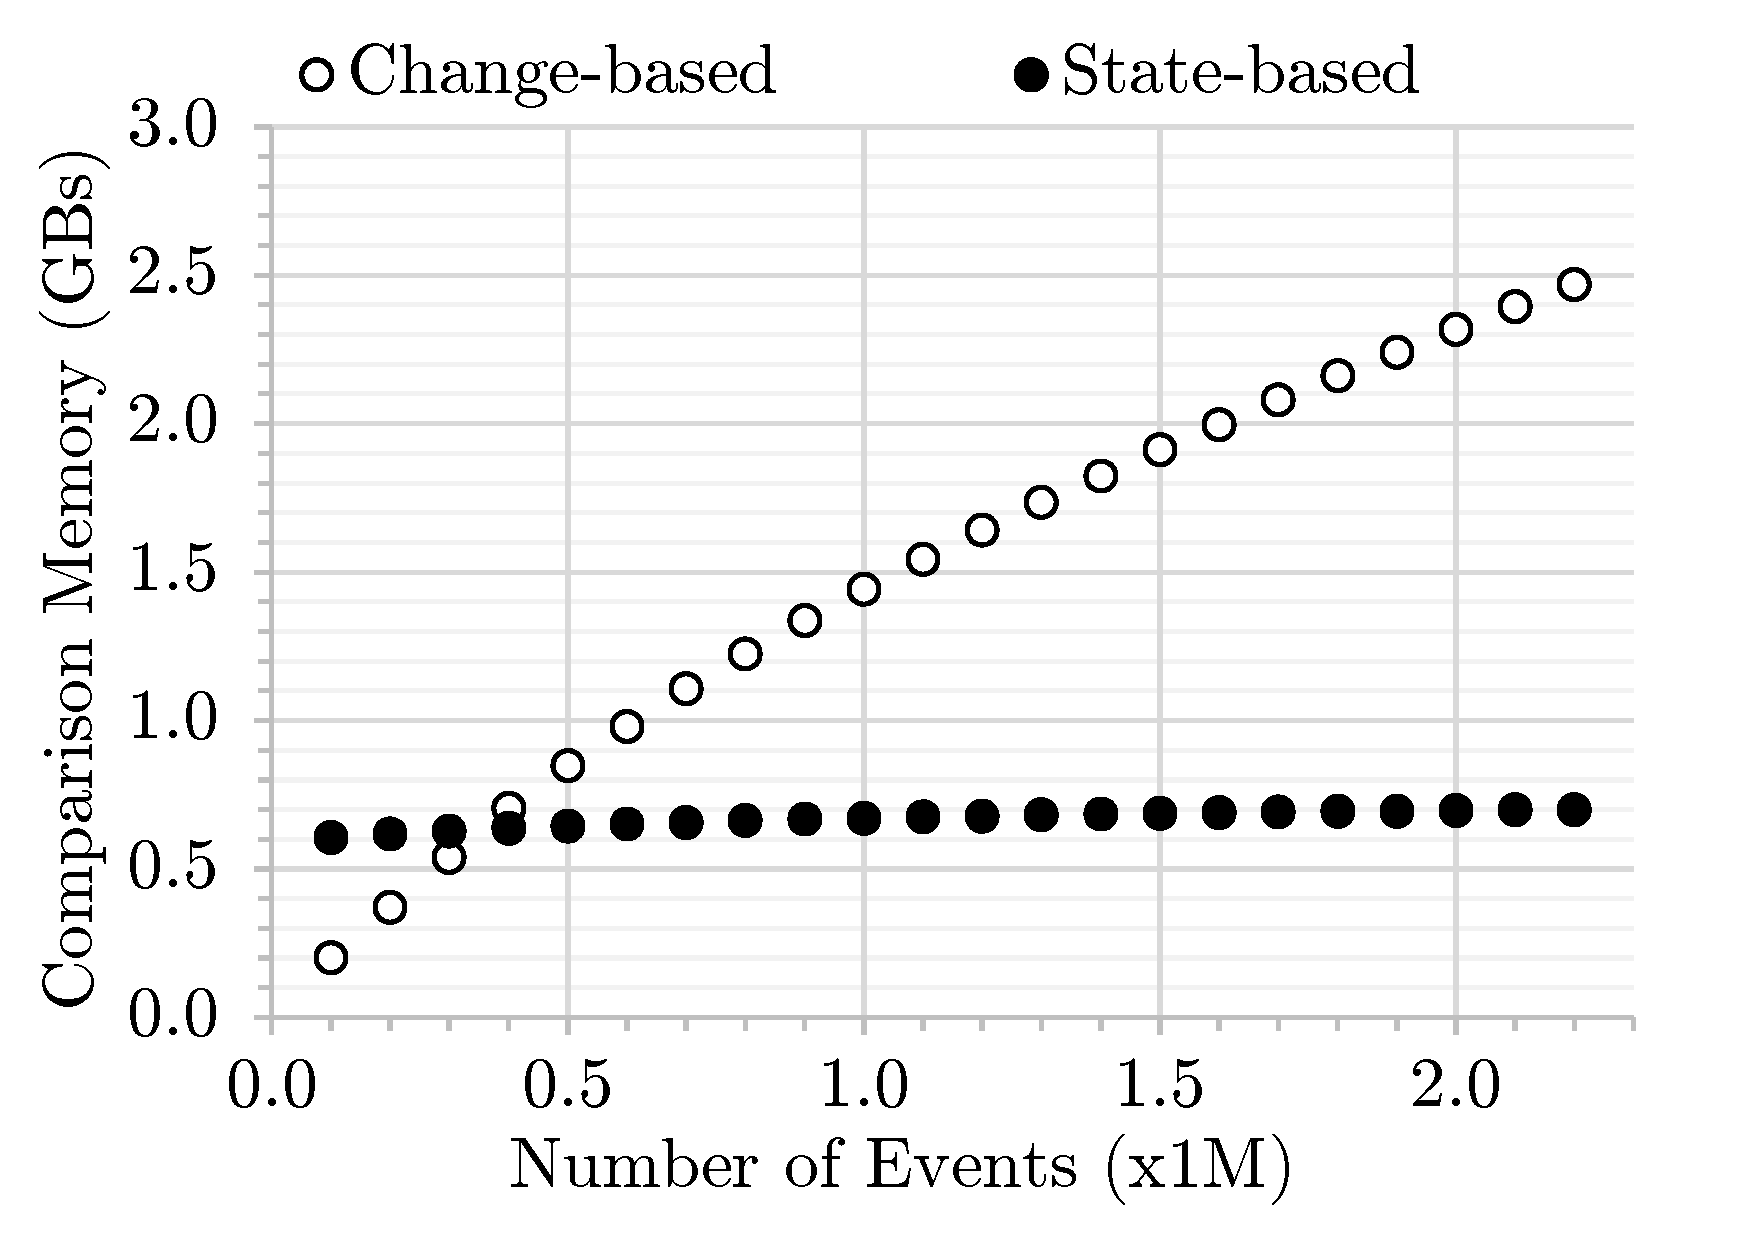
\includegraphics[width=\linewidth]{change-memory-events}
    \caption{change-only}
    \label{fig:change-memory-events}
  \end{subfigure}
  \caption{Memory footprint for homogeneous operations.}
  \label{fig:operation_memory_events}
\end{figure}

Figures \ref{fig:operation_time_events} and \ref{fig:operation_memory_events} show the comparison times and memory footprints of models modified using homogeneous operations—\textsf{add}, \textsf{remove}, \textsf{move}, or \textsf{set} only. In all these figures, change-based comparison outperforms its state-based counterpart, particularly when the number of change events is small relative to the size of the model. As the number of modifications grows, change-based comparison becomes slower than state-based comparison. In our experiments, this happens when the number of events is greater than 4 million (Figure \ref{fig:add-time-events}). Change-based comparison also becomes slower when the size of models shrinks (because of a large number of delete events) as depicted in Figure \ref{fig:delete-memory-events}. This is because change-based comparison still needs to load these change events and construct its element tree. In contrast, deletion means less work for state-based comparison. In terms of memory footprint, change-based comparison performs better than state-based comparison only when the number of change events is fewer than 0.3 million, as depicted in Figure \ref{fig:operation_memory_events}.




\section{Conclusions}
\label{sec:conclusions_6}
This chapter proposed an approach to identify differences between two versions of a model persisted in change-based format. It works by loading into memory the changes made to both versions since the last shared version, constructing partial states of the versions based on the information in the latest changes, and using specific rules to identify differences between the versions’ elements and features.

The evaluation indicates that the change-based comparison approach works best for large models that have been modified a moderate number of times. Models that have been modified excessively and experience a significant reduction in size could impair the performance of change-based model differencing, since a high number of change records must be read and loaded into memory.

This chapter has addressed the second research question of this study, \textbf{In a changed-based format, how can the differences between models be identified, and how does change-based model differencing perform, in terms of speed and memory footprint, compared to state-based model differencing?} (RQ2). Change-based persistence can identify differences between two versions of a model. The change-based representation of the two versions contains all the information needed to identify elements that have been modified since their last shared version. In this way, we can localise the model differencing to the elements that were modified recently. In other words, it is not necessary to inspect, match, and diff all the elements. We can reconstruct the partial states of the two versions and then compare their elements and features using specific rules to identify their differences.

The change-based model differencing proposed in this research comprises three phases: event loading, element tree construction, and diff computation. In the event loading phase, the implementation loadfpds change events recorded in two change-based model persistence files into memory starting from the line their change events are different. The information that the loaded change events contain is used to construct an element tree. An element tree contains only the affected elements and features of the versions being compared, including the shared original version. This is possible because change events are designed to contain adequate information to construct the element tree. A diff computation is then executed to identify the differences using a set of pre-defined rules (i.e., if an element is created in one version it means that the element does not exist in the other version or in the original version).

The evaluation suggests that the proposed change-based model differencing executes faster than traditional, state-based model differencing.
However, change-based model differencing needs to load change events from a change-based persistence into main memory. Thus, it may require more memory than is needed for state-based model differencing. In our evaluation, this occurs when the number of change events exceeds 400,000. However, it is likely that diff and merge operations are performed on lower numbers of changes (smaller deltas) than were tested in this evaluation.

